\documentclass[12pt,a4paper]{article}

\usepackage{fontspec}
\setmainfont{TeX Gyre Pagella}

\usepackage{amsmath,amssymb}
\usepackage{amsthm}
\usepackage{geometry}
\usepackage{setspace}
\usepackage{hyperref}
\usepackage{microtype}
\usepackage{tikz}
\usetikzlibrary{arrows.meta,positioning,calc,decorations.pathmorphing}

\geometry{margin=1.2in}
\onehalfspacing

\newtheorem{theorem}{Theorem}
\newtheorem{corollary}{Corollary}[theorem]

\title{Against Indiscriminate Visibility:\\
On the Structural Risks of Virality, Publicity, and Exposure}
\author{Flyxion}
\date{\today}

\begin{document}

\maketitle

\begin{abstract}
Contemporary digital culture treats visibility as an intrinsic good and virality as a desirable objective. This essay argues that indiscriminate exposure is structurally unstable and often counterproductive. Increasing visibility expands not only opportunity, but also adversarial surface area, interpretive distortion, and reputational fragility. Without institutional backing, legal protection, or social insulation, individuals who seek rapid publicity may expose themselves to asymmetric harms that are difficult or impossible to defend against. The analysis proceeds by examining the asymmetry between rumor and truth, the incentives of local and institutional actors, and the mismatch between exposure and resilience. These informal observations are subsequently formalized within the scalar--vector--entropy framework of the Relativistic Scalar--Vector Plenum (RSVP), culminating in a variational principle, a no-go theorem for safe virality, and a set of design implications for systems that must manage visibility under entropic constraints.
\end{abstract}

\newpage

\section{Introduction}

The dominant paradigm of online and entrepreneurial culture encourages individuals to maximize reach: to ``build an audience,'' ``go viral,'' and ``get attention.'' This paradigm assumes that attention scales linearly with benefit. However, attention is not a neutral resource. It is a field of interaction populated by agents with heterogeneous incentives, including indifference, opportunism, and hostility.

To increase visibility is therefore not merely to increase opportunity, but to increase the number of observers capable of acting upon one's reputation, work, and identity. In the absence of corresponding increases in protection, this produces a structural imbalance. The mistake embedded in virality culture is treating exposure as a monotonically beneficial quantity, when in practice it behaves more like an unstable phase transition: below certain thresholds, largely inert; above them, rapidly amplifying both positive and negative dynamics, with the negative dynamics typically scaling more aggressively.

This essay proceeds from informal observation to formal model. The early sections establish the qualitative asymmetries involved. The later sections embed these asymmetries within the RSVP field-theoretic framework, where they become consequences of coupled scalar--vector--entropy dynamics rather than contingent social observations.

\section{The Asymmetry Between Rumor and Truth}

Truth is typically slow, constrained, and evidential. It requires time, context, and verification. Rumor, by contrast, is fast, unconstrained, and transmissible at low cost.

This asymmetry can be informally expressed as:
\[
\text{Propagation}_{\text{rumor}} \gg \text{Propagation}_{\text{truth}}
\]

More importantly, correction does not scale proportionally with falsehood. A single unverified claim may require extensive effort to refute, and even then, the refutation rarely reaches all recipients of the original claim. The asymmetry is not merely quantitative but structural: the conditions that make a claim easy to spread---emotional salience, narrative simplicity, compatibility with existing suspicion---are precisely the conditions that make it difficult to dislodge.

Thus, as visibility increases, the rumor surface grows faster than the truth surface. The system becomes increasingly dominated by narratives that are easier to spread than to correct. An individual who increases their exposure without increasing their capacity for narrative correction has therefore degraded their expected informational environment, not improved it.

\begin{figure}[htbp]
\centering
\begin{tikzpicture}[scale=1.1]
\draw[->] (0,0) -- (6,0) node[right] {$t$};
\draw[->] (0,0) -- (0,4) node[above] {Propagation};
\draw[thick] (0,0) .. controls (2,1.2) and (4,2.2) .. (5.5,2.8)
  node[right] {\small truth};
\draw[thick,dashed] (0,0) .. controls (1,2) and (3,3.2) .. (5.5,3.6)
  node[right] {\small rumor};
\end{tikzpicture}
\caption{Propagation asymmetry: rumor spreads faster and saturates at higher amplitude than truth. Correction effort scales with the gap between the two curves.}
\end{figure}

\section{Reputational Attack Surfaces}

Visibility expands what may be called the reputational attack surface: the set of individuals who can interpret, misinterpret, or deliberately distort one's actions and statements.

In small offline communities, this may manifest as gossip, informal sanctions, or exclusion. In larger networks, it may include defamation, coordinated harassment, or reputational framing. Crucially, these processes often operate below formal thresholds of accountability. They are difficult to litigate, difficult to trace, and difficult to disprove. Without access to legal resources, institutional legitimacy, or defensive infrastructure, individuals are structurally disadvantaged.

It is worth noting that these dynamics do not require bad actors in any unusual sense. Most of the agents who contribute to reputational degradation are acting from entirely ordinary motives: self-protection, community cohesion, or the casual transmission of interesting information. The structure of the damage does not depend on the presence of malice; it depends only on the presence of a large enough audience and the absence of corrective capacity.

\begin{figure}[htbp]
\centering
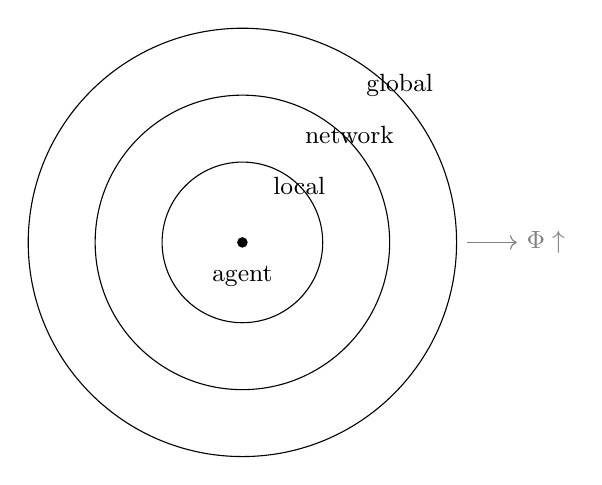
\begin{tikzpicture}[scale=0.85]
\draw[fill=black] (0,0) circle (0.07);
\node[below=5pt] at (0,0) {\small agent};
\draw (0,0) circle (1.2);
\draw (0,0) circle (2.2);
\draw (0,0) circle (3.2);
% labels on the arcs at 45 degrees to avoid overlap
\node at (0.85,0.85) {\small local};
\node at (1.6,1.6) {\small network};
\node at (2.35,2.35) {\small global};
% arrow outside
\draw[->,gray] (3.35,0) -- (4.1,0) node[right] {\small $\Phi\uparrow$};
\end{tikzpicture}
\caption{Expanding visibility expands the reputational attack surface nonlinearly. Each ring represents a new class of observers capable of acting on an agent's reputation.}
\end{figure}

\section{Lack of Defensive Infrastructure}

Established actors---corporations, universities, governments---possess layers of defense: legal teams, public relations departments, internal networks of trust, and mechanisms for narrative control. Individuals typically possess none of these.

This creates a mismatch:
\[
\text{Exposure} \uparrow \quad \text{without} \quad \text{Defense} \uparrow
\]

When exposure increases without a corresponding increase in defensive capacity, vulnerability increases nonlinearly. The individual becomes legible to many, but protected by few.

The institutional defenses available to large actors are not merely quantitatively greater than those available to individuals; they are qualitatively different in kind. A corporation that faces a defamatory claim can deploy legal pressure, issue coordinated statements across multiple channels, and absorb reputational damage while the issue is resolved. An individual faces these same attacks with personal time, limited credibility, and no institutional amplification. Scaling exposure without scaling defense is therefore not merely risky but structurally disadvantageous.

\section{Local Incentives and Social Stability}

Public expression does not occur in a vacuum. It interacts with local systems of belief, identity, and social reproduction.

In many cases, individuals embedded in these systems will interpret novel or disruptive ideas not as neutral contributions, but as threats to coherence. This response does not require malice; it follows from the role such systems play in maintaining meaning and stability. A community organized around a particular religious, ideological, or cultural framework perceives expressions that challenge that framework not as intellectual invitations but as existential provocations. The reaction is accordingly defensive rather than evaluative.

As a result, attempts at broad dissemination may trigger defensive reactions at the level of individuals and communities. These reactions can include rejection, mischaracterization, or active opposition. The individual who broadcasts into these contexts without calibrating for interpretive compatibility will encounter resistance that is entirely predictable from the structure of the interaction, regardless of the quality or accuracy of what they are communicating.

\section{Adversarial Incentives}

Not all opposition is defensive. Some actors have direct incentives to resist or undermine new entrants.

If an individual produces a cheaper, more efficient, or more accessible alternative to an existing product or idea, incumbent actors may experience this as a loss. The rational response, in many cases, is not cooperation but resistance. This resistance need not be formal or coordinated. It may manifest as subtle discouragement, reputational framing, or the amplification of negative narratives. Individuals who attempt to correct harmful behavior or expose ongoing misconduct face analogous dynamics: those whose interests are threatened will not respond with gratitude but with counter-pressure.

Similarly, individuals embedded in systems of relative evaluation---where one agent's success reduces others' standing---face structural incentives for adversarial interpretation that operate independently of personal animosity. The topology of the evaluation system produces the conflict; the participants are largely executing what the structure incentivizes.

\section{The Nonlinearity of Exposure}

A key misunderstanding in virality strategies is the assumption of linear scaling: that doubling visibility doubles benefit.

In reality, exposure often exhibits threshold behavior. Below a certain level, visibility produces minimal effects. Above a threshold, it produces rapid amplification of both positive and negative dynamics. However, the negative dynamics---misinterpretation, rumor, adversarial attention---often scale more aggressively than the positive ones. The positive outcomes of visibility are frequently diffuse, probabilistic, and delayed. The negative outcomes are concentrated, immediate, and self-amplifying.

Thus, beyond a certain point:
\[
\frac{d(\text{risk})}{d(\text{visibility})} > \frac{d(\text{benefit})}{d(\text{visibility})}
\]

The inflection at which this inequality becomes binding varies by context, but under conditions of limited defensive capacity, it tends to occur well before the scales of exposure that virality culture treats as targets.

\begin{figure}[htbp]
\centering
\begin{tikzpicture}
\draw[->] (0,0) -- (6,0) node[right] {$\Phi$};
\draw[->] (0,0) -- (0,4) node[above] {Effect};
\draw[thick] (0,0) .. controls (2,1) and (4,1.6) .. (5.5,2)
  node[right] {\small benefit};
\draw[thick,dashed] (0,0) .. controls (2,1.2) and (3.5,3.2) .. (5.5,4)
  node[right] {\small risk};
\draw[dotted] (2.8,0) -- (2.8,2.1);
\node[below] at (2.8,0) {\small $\Phi_c$};
\end{tikzpicture}
\caption{Risk grows superlinearly relative to benefit beyond the critical threshold $\Phi_c$. Below $\Phi_c$ the two curves are comparable; above it, risk dominates.}
\end{figure}

\section{Indiscriminate vs.\ Selective Dissemination}

The central problem is not visibility itself, but indiscriminate visibility.

Selective dissemination---sharing work within contexts where it can be understood, evaluated, and supported---allows for alignment between exposure and resilience. When an audience possesses the interpretive context to engage with a claim on its own terms, entropy production is reduced. When an audience lacks that context, or when its incentives run counter to the claim's reception, interpretation diverges from intention and entropy accumulates.

Indiscriminate dissemination maximizes reach without regard for interpretive compatibility or defensive capacity. It exposes work to audiences that may lack the context, incentives, or goodwill necessary for constructive engagement. The result is not merely inefficiency but instability: the signal degrades faster than it can be transmitted.

\section{A Field-Theoretic Model of Visibility and Reputational Dynamics}

We now formalize the dynamics of publicity using a field-theoretic perspective aligned with scalar--vector--entropy frameworks.

Let:
\[
\Phi(x,t) \quad \text{denote the visibility (exposure) field}
\]
\[
\mathbf{v}(x,t) \quad \text{denote the interpretive flow field}
\]
\[
S(x,t) \quad \text{denote reputational entropy (distortion, uncertainty, rumor density)}
\]

Here, $x$ indexes a social or informational manifold (e.g., audiences, communities, or network regions), and $t$ denotes time.

\subsection{Visibility as a Scalar Potential}

Visibility behaves as a scalar potential that attracts interpretive flows:
\[
\mathbf{v} \sim \nabla \Phi + \boldsymbol{\xi}
\]
where $\boldsymbol{\xi}$ represents stochastic or adversarial perturbations.

As $\Phi$ increases, gradients steepen, and more agents are drawn into interaction. However, these flows are not uniformly aligned; they include misunderstanding, opportunism, and hostility.

\subsection{Entropy Production and Rumor Amplification}

Reputational entropy evolves according to a balance equation:
\[
\frac{\partial S}{\partial t}
=
\alpha |\mathbf{v}|^2
-
\beta \, \mathcal{C}(\Phi)
\]

The first term captures entropy production from interpretive activity: the more attention and interaction, the greater the potential for distortion.

The second term represents corrective capacity $\mathcal{C}(\Phi)$, which depends on available resources such as credibility, institutional support, and communication bandwidth.

For most individuals:
\[
\mathcal{C}(\Phi) \ll |\mathbf{v}|^2 \quad \text{as } \Phi \to \text{large}
\]

Thus:
\[
\frac{\partial S}{\partial t} > 0
\]
indicating net growth of distortion with increased visibility.

\subsection{Rumor as Low-Energy Propagation}

Rumor can be modeled as a low-energy excitation of the entropy field:
\[
\text{Cost}_{\text{rumor}} \ll \text{Cost}_{\text{verification}}
\]

This produces an asymmetry analogous to thermodynamic irreversibility: once entropy increases, it is costly to reverse. In this sense, reputational dynamics exhibit a form of coarse-grained irreversibility:
\[
S(t_2) \geq S(t_1) \quad \text{for } t_2 > t_1
\]
unless significant external work is applied.

\subsection{Exposure Without Protection as Instability}

Define a protection functional $P(\Phi)$ capturing legal, institutional, and social defenses.

Stability requires:
\[
P(\Phi) \gtrsim S(\Phi)
\]

However, for individuals:
\[
P(\Phi) \approx \text{constant}, \quad S(\Phi) \uparrow
\]

Thus there exists a critical visibility $\Phi_c$ such that:
\[
S(\Phi_c) > P(\Phi_c)
\]

Beyond this threshold, the system enters an unstable regime where reputational degradation dominates corrective capacity.

\subsection{Adversarial Vector Fields}

Not all interpretive flow is neutral. Introduce a decomposition:
\[
\mathbf{v} = \mathbf{v}_{\text{benign}} + \mathbf{v}_{\text{adversarial}}
\]

Adversarial components may be driven by economic competition, ideological conflict, social signaling, or opportunistic exploitation. These components are often amplified by visibility gradients, leading to nonlinear effects such as coordinated attacks or cascade failures in reputation.

\subsection{Selective Coupling and Boundary Conditions}

Let $D \subseteq \mathcal{M}$ denote a domain of aligned or high-context audiences.

Restricting exposure corresponds to imposing boundary conditions:
\[
\Phi(x,t) = 0 \quad \text{for } x \notin D
\]

Within $D$, interpretive flows are more coherent, and entropy production is reduced:
\[
\alpha_D < \alpha_{\text{global}}
\]

Thus selective dissemination acts as a form of entropy control.

\subsection{Nonlinear Risk Scaling}

Define total risk $R(\Phi)$ as a functional of entropy and adversarial flow:
\[
R(\Phi) = \int \left( S + \gamma |\mathbf{v}_{\text{adversarial}}| \right) dx
\]

Empirically and structurally, this satisfies:
\[
\frac{dR}{d\Phi} \quad \text{increases with } \Phi
\]

Thus risk scales superlinearly with exposure.

\begin{figure}[htbp]
\centering
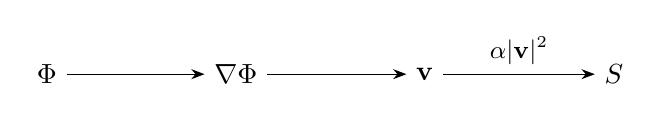
\begin{tikzpicture}[node distance=2.4cm,>=Stealth]
\node (phi) {$\Phi$};
\node (grad) [right of=phi] {$\nabla\Phi$};
\node (v)    [right of=grad] {$\mathbf{v}$};
\node (S)    [right of=v]    {$S$};
\draw[->] (phi) -- (grad);
\draw[->] (grad) -- (v);
\draw[->] (v) -- node[above]{\small $\alpha|\mathbf{v}|^2$} (S);
\end{tikzpicture}
\caption{Core mechanism of the field model: visibility gradients induce interpretive flow, and flow produces reputational entropy at rate $\alpha|\mathbf{v}|^2$.}
\end{figure}

\begin{figure}[htbp]
\centering
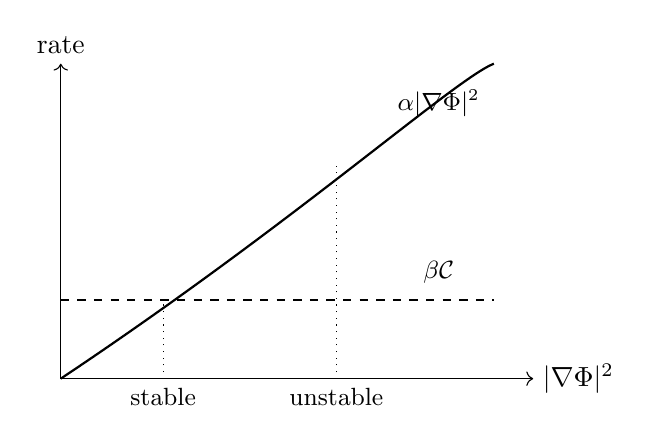
\begin{tikzpicture}
\draw[->] (0,0) -- (6,0) node[right] {$|\nabla\Phi|^2$};
\draw[->] (0,0) -- (0,4) node[above] {rate};
\draw[thick] (0,0) .. controls (3,2) and (5,3.8) .. (5.5,4);
\node at (4.8,3.5) {\small $\alpha|\nabla\Phi|^2$};
\draw[thick,dashed] (0,1) -- (5.5,1);
\node at (4.8,1.35) {\small $\beta\mathcal{C}$};
\draw[dotted] (1.3,0) -- (1.3,1);
\node[below] at (1.3,0) {\small stable};
\draw[dotted] (3.5,0) -- (3.5,2.7);
\node[below] at (3.5,0) {\small unstable};
\end{tikzpicture}
\caption{Entropy production $\alpha|\nabla\Phi|^2$ grows without bound while corrective capacity $\beta\mathcal{C}$ is bounded. Instability begins where the curves cross.}
\end{figure}

\section{Universality of Exposure Across Domains}

The dynamics described above are not specific to digital platforms or social media. Any act that increases legibility within a social field contributes to the visibility function $\Phi(x,t)$.

This includes publishing books or essays, exhibiting art, giving interviews or lectures, introducing new products or pricing models, or publicly criticizing institutions. In each case, the mechanism is identical: the agent increases coupling to a broader interpretive environment. The medium changes, but the field dynamics do not.

\subsection{Moral Alignment Does Not Confer Protection}

A common assumption is that adherence to ethical norms, factual accuracy, or good intentions provides protection against reputational harm.

Within the present framework, this assumption does not hold. The evolution of reputational entropy $S$ depends on interpretive flows and incentives, not on the intrinsic truth value of the signal. Formally, correctness is not a stabilizing term in the entropy equation:
\[
\frac{\partial S}{\partial t}
\neq f(\text{truth})
\]

Instead, entropy production is driven by interaction density and interpretive heterogeneity. As a result, even morally aligned or factually correct contributions may generate high entropy under sufficient exposure.

\subsection{Opacity of Suppression Mechanisms}

Modern dissemination systems introduce additional structure in the form of algorithmic mediation. Let $A(x,t)$ denote an amplification operator governing the visibility field.

Then:
\[
\Phi_{\text{effective}} = A(x,t)\,\Phi
\]

In many cases, $A$ is partially opaque. This introduces two asymmetries: agents cannot directly observe whether their visibility is being attenuated or amplified, and observed successes may not reflect underlying accessibility, but selective amplification. This opacity produces the appearance that certain individuals ``slip through,'' while others do not, without revealing the governing selection criteria.

\subsection{Decoy Amplification and Narrative Containment}

Let $N(x,t)$ denote the narrative space of publicly circulating ideas.

Not all ideas propagate equally. In some cases, highly visible arguments function as attractors that absorb attention while leaving more structurally disruptive arguments unexpressed or marginalized. This can be modeled as a redistribution of attention density:
\[
\int_{N} \Phi \, dx = \text{constant}, \quad \text{but concentrated on a subset } N'
\]

where $N'$ consists of arguments that are compatible with existing interpretive or institutional structures. In this sense, apparent visibility may coexist with containment.

\subsection{Economic Disruption and Local Adversarial Response}

Consider a simple example: an agent introduces a product with drastically lower cost.

Let $C_{\text{market}}$ denote the prevailing cost structure, and $C_{\text{new}} \ll C_{\text{market}}$.

This creates a gradient:
\[
\nabla C < 0
\]

Such a gradient induces adversarial flows from incumbent actors whose stability depends on the existing cost structure. These flows may include reputational framing, regulatory pressure, informal discouragement, or coordinated exclusion. Importantly, these responses do not require explicit coordination. They arise from aligned incentives within the field.

\subsection{Relative Evaluation Systems and Induced Adversarial Flow}

Consider a system in which outcomes are assigned relative to a population, such as grading on a curve.

Let $p_i$ denote the performance of agent $i$, and let rank $r_i$ be determined by the distribution:
\[
r_i = F(p_i \mid \{p_j\})
\]

where $F$ depends on the entire set of performances. In such systems:
\[
\frac{\partial r_j}{\partial p_i} < 0 \quad \text{for } i \neq j
\]

That is, an increase in one agent's performance reduces the relative standing of others.

This creates a coupling between agents: $p_i \uparrow$ implies $r_j \downarrow$, even when $p_j$ is unchanged. Thus, improvement by one agent generates a negative externality for others. This induces adversarial interpretive flow:
\[
\mathbf{v}_{\text{adversarial}} \sim \nabla r
\]

where gradients in rank produce comparison, blame, and reputational tension. Any system that evaluates agents relatively rather than absolutely introduces coupling of this form, including grading curves, rankings, competitive markets, and attention economies. Resentment in such systems is not primarily a moral failure of individuals, but a consequence of the evaluation topology.

\subsection{Cross-Institutional Coupling}

Economic, social, and cultural systems are not independent. A perturbation in one domain propagates across others:
\[
\delta \Phi_{\text{economic}} \rightarrow \delta \mathbf{v}_{\text{social}} \rightarrow \delta S_{\text{reputational}}
\]

Thus even a localized innovation can trigger distributed responses across multiple layers of the system.

\section{Control Theory of Visibility: Regulating Exposure Under Entropic Constraints}

The preceding analysis establishes that visibility $\Phi$ is not intrinsically beneficial, but a driver of entropy production and adversarial interaction. We now treat visibility as a control variable to be regulated over time.

\subsection{State Variables and Objective}

Let the system state be given by:
\[
(\Phi, \mathbf{v}, S, P)
\]
where $\Phi$ is visibility, $\mathbf{v}$ interpretive flow, $S$ reputational entropy, and $P$ protective capacity.

Define an objective functional:
\[
\mathcal{J} = \int \left( U(\Phi) - \lambda S - \mu R \right) dt
\]
where $U(\Phi)$ represents utility gained from visibility, $S$ is entropy (distortion), $R$ is adversarial risk, and $\lambda, \mu > 0$ are weighting parameters.

The goal is not to maximize $\Phi$, but to maximize $\mathcal{J}$ under dynamical constraints.

\subsection{Critical Visibility Threshold}

As established, there exists a critical threshold $\Phi_c$ such that:
\[
S(\Phi_c) \approx P(\Phi_c)
\]

Define the admissible region $\Phi < \Phi_c$. Control policy must ensure the system remains within this region. Crossing $\Phi_c$ induces instability, where entropy growth outpaces defensive capacity.

\subsection{Visibility as a Controlled Input}

Let $u(t)$ denote the rate of exposure (publishing, broadcasting, distribution effort).

Then:
\[
\frac{d\Phi}{dt} = u(t) - \delta \Phi
\]
where $\delta$ represents natural decay of attention. The control problem is to choose $u(t)$ such that $\Phi(t) \in [0, \Phi_c)$.

\subsection{Domain-Restricted Dissemination}

Let $D(t)$ be the active audience domain.

Restricting exposure corresponds to:
\[
u(t) = u_D(t), \quad D \subset \mathcal{M}
\]

The optimal strategy is not global broadcasting but controlled expansion:
\[
D_1 \subset D_2 \subset \cdots \subset \mathcal{M}
\]

with each expansion contingent on stability:
\[
S(D_k) < P(D_k)
\]

This produces a staged growth process rather than instantaneous virality.

\subsection{Entropy Budgeting}

Define an entropy budget $S(t) \leq S_{\max}$.

Each act of exposure consumes part of this budget:
\[
\Delta S \sim \alpha |\mathbf{v}|^2 \Delta t
\]

Thus publication and publicity must be treated as expenditures, not free actions. High-frequency or high-amplitude exposure rapidly depletes the entropy budget, leading to loss of control over narrative dynamics.

\subsection{Adaptive Feedback Control}

Introduce a feedback policy:
\[
u(t) = f\big(S(t), R(t), P(t)\big)
\]

A simple stabilizing controller is:
\[
u(t) =
\begin{cases}
u_0 & \text{if } S \ll P \\
0 & \text{if } S \approx P \\
-\kappa & \text{if } S > P
\end{cases}
\]

where $-\kappa$ represents active withdrawal (reducing visibility, disengaging channels). Thus, exposure is reduced or halted when instability is detected.

\begin{figure}[htbp]
\centering
\begin{tikzpicture}[node distance=2.4cm,>=Stealth]
\node (u)       {$u(t)$};
\node (phi)     [right of=u]    {$\Phi$};
\node (flow)    [right of=phi]  {$\mathbf{v}$};
\node (entropy) [right of=flow] {$S$};
\node (ctrl)    [below of=phi,yshift=0.4cm]  {$f(S,P)$};
\draw[->] (u) -- (phi);
\draw[->] (phi) -- (flow);
\draw[->] (flow) -- (entropy);
\draw[->] (entropy.south) .. controls +(0,-0.8) and +(1.2,0) .. (ctrl.east);
\draw[->] (ctrl.west) .. controls +(-1.2,0) and +(0,-0.8) .. (u.south);
\end{tikzpicture}
\caption{Feedback control of visibility. Entropy $S$ feeds back through the controller $f(S,P)$ to modulate the exposure input $u(t)$, maintaining the system below the critical threshold.}
\end{figure}

\subsection{Latency and Recovery}

Entropy reduction is slower than entropy production:
\[
\left|\frac{dS}{dt}\right|_{\text{decay}} \ll \left|\frac{dS}{dt}\right|_{\text{growth}}
\]

Therefore, recovery requires extended periods of low or zero exposure:
\[
u(t) \approx 0 \quad \text{for } t \in [t_1, t_2]
\]

This explains why reputational repair is time-intensive and why rapid re-exposure often worsens instability.

\subsection{Stealth and Low-Gradient Strategies}

An alternative regime is to maintain:
\[
\nabla \Phi \approx 0
\]

This corresponds to low-gradient visibility: remaining below detection thresholds of large-scale adversarial flows while still enabling local interaction. In this regime, growth occurs through dense local networks, repeated small-scale interactions, and high-context communication. Rather than maximizing reach, the system maximizes coherence.

\section{The Visibility Minimization Principle and Reputational Irreversibility}

We now introduce a variational principle governing exposure in systems subject to asymmetric information dynamics.

\subsection{Statement of the Principle}

Let $\Phi(t)$ denote the visibility trajectory of an agent over time, and let $\mathcal{T}$ denote a task, objective, or communicative function.

\medskip

\noindent
\textbf{Visibility Minimization Principle.}
\emph{Among all trajectories that successfully realize $\mathcal{T}$, the optimal trajectory minimizes cumulative visibility:}
\[
\Phi^\ast = \arg\min_{\Phi \in \mathcal{A}(\mathcal{T})} \int_{t_0}^{t_1} \Phi(t)\,dt
\]

\medskip

Here, $\mathcal{A}(\mathcal{T})$ is the admissible set of trajectories that achieve the objective. This principle asserts that visibility is not a resource to be maximized, but a cost to be minimized, analogous to action in classical mechanics.

\subsection{Augmented Action Functional}

Define an effective action:
\[
\mathcal{S}_{\text{eff}}[\Phi] = \int \left( L_{\text{task}} - \lambda \Phi - \mu S \right) dt
\]

where $L_{\text{task}}$ encodes progress toward the objective, $\Phi$ is visibility, $S$ is reputational entropy, and $\lambda, \mu > 0$ are cost coefficients.

Optimal trajectories satisfy:
\[
\delta \mathcal{S}_{\text{eff}} = 0
\]

This produces Euler--Lagrange dynamics in which increases in visibility must be justified by proportional gains in task completion.

\subsection{Reputational Entropy as a Non-Conserved Quantity}

Unlike energy in closed physical systems, reputational entropy is not conserved. It is generically produced under interaction:
\[
\frac{dS}{dt} = \alpha |\mathbf{v}|^2 - \beta \mathcal{C}
\]

with $\alpha > 0$ and $\mathcal{C}$ representing corrective capacity.

For most agents, $\beta \mathcal{C} \ll \alpha |\mathbf{v}|^2$, thus:
\[
\frac{dS}{dt} > 0
\]

indicating irreversible growth under exposure.

\subsection{Irreversibility and Path Dependence}

Let $S(t)$ be coarse-grained reputational entropy. Then for typical trajectories:
\[
S(t_2) \geq S(t_1), \quad t_2 > t_1
\]

This induces path dependence: early exposure decisions constrain future states. In particular, high initial visibility creates residual entropy that cannot be fully eliminated, only redistributed or diluted.

\subsection{Noether-Like Tradeoff Relation}

Consider a transformation that increases visibility:
\[
\Phi \rightarrow \Phi + \delta \Phi
\]

This induces a corresponding increase in entropy:
\[
\delta S \geq k \, \delta \Phi
\]

for some $k > 0$ determined by the interaction structure. Thus we obtain a tradeoff relation:
\[
\frac{dS}{d\Phi} \geq k
\]

This functions analogously to a conservation constraint: increases in visibility necessarily generate entropy beyond a minimum rate.

\subsection{Gauge Interpretation of Visibility}

Visibility can be interpreted as a gauge-like degree of freedom in the communicative field. Different representations of the same underlying work may correspond to different $\Phi$-configurations. However, high-$\Phi$ gauges couple more strongly to adversarial flows.

A low-visibility gauge minimizes coupling while preserving internal structure:
\[
\text{Observable output invariant, but } \Phi \downarrow
\]

Thus, gauge choice affects stability even when content remains unchanged.

\subsection{Decoupling and Hidden Manifolds}

Let $D \subset \mathcal{M}$ denote a restricted domain of interaction.

Define a decoupled manifold where:
\[
\Phi(x) \approx 0 \quad \text{for } x \notin D
\]

Within $D$, meaningful interaction can occur without inducing global entropy cascades. This corresponds to performing work in a partially hidden or low-coupling regime, only projecting outward when necessary.

\subsection{Corollary: Virality as Action Divergence}

Uncontrolled virality corresponds to trajectories where:
\[
\int \Phi(t)\,dt \to \infty \quad \text{over short intervals}
\]

In such cases, the entropy term dominates:
\[
\mathcal{S}_{\text{eff}} \to -\infty
\]

indicating a breakdown of stable dynamics. Thus virality is not merely high exposure, but divergence from optimal action.

\section{Reputational Dynamics as a Sector of the Relativistic Scalar--Vector Plenum}

We now demonstrate that the dynamics of visibility, interpretation, and reputational entropy are not merely analogous to field-theoretic systems, but constitute a concrete instantiation of the scalar--vector--entropy structure within the Relativistic Scalar--Vector Plenum (RSVP).

\subsection{Manifold of Interpretation}

Let $\mathcal{M}$ denote a manifold of observers, contexts, or interpretive loci. Each point $x \in \mathcal{M}$ represents a local configuration of beliefs, incentives, and informational access. Fields defined over $\mathcal{M}$ encode the state of an agent's presence within this manifold.

\subsection{Field Identification}

We identify:
\[
\Phi(x,t) \equiv \text{visibility density}
\]
\[
\mathbf{v}(x,t) \equiv \text{interpretive transport (narrative flow)}
\]
\[
S(x,t) \equiv \text{reputational entropy density}
\]

These correspond directly to the scalar, vector, and entropy fields of RSVP.

\subsection{Field Equations}

The coupled dynamics take the form:

\paragraph{Scalar (Visibility) Evolution}
\[
\frac{\partial \Phi}{\partial t}
+ \nabla \cdot (\Phi \mathbf{v})
=
u - \delta \Phi
\]

where $u$ is intentional exposure (publication, broadcast) and $\delta$ is decay.

\paragraph{Vector (Interpretive Flow) Evolution}
\[
\frac{\partial \mathbf{v}}{\partial t}
=
- \nabla \Phi
- \nabla S
+ \mathbf{F}_{\text{ext}}
\]

The flow is driven by gradients in visibility (attention attraction) and entropy (uncertainty, controversy), along with external forcing (economic, ideological, institutional pressures).

\paragraph{Entropy (Reputation) Evolution}
\[
\frac{\partial S}{\partial t}
+ \nabla \cdot (S \mathbf{v})
=
\alpha |\mathbf{v}|^2
- \beta \mathcal{C}
\]

Entropy is advected by interpretive flow and produced by interaction intensity, while reduced by corrective capacity $\mathcal{C}$.

\subsection{Lamphrodyne Smoothing Interpretation}

Within RSVP, high-entropy gradients induce smoothing flows (lamphrodyne relaxation). In the reputational sector, this manifests as attempts to resolve ambiguity or restore coherence. However, unlike physical systems, corrective capacity is limited and unevenly distributed:
\[
\beta \mathcal{C}(x,t) \ll \alpha |\mathbf{v}|^2
\]

Thus smoothing is incomplete, and residual entropy persists.

\subsection{Torsion and Narrative Distortion}

Non-integrable circulation in the vector field corresponds to narrative torsion:
\[
\nabla \times \mathbf{v} \neq 0
\]

This produces loops of reinterpretation, contradiction, and feedback, in which statements are reframed and reintroduced in altered forms. Such torsion is amplified by high visibility gradients and heterogeneous interpretive contexts.

\subsection{Constraint Structure and Stability}

Define a stability condition:
\[
S(x,t) \leq P(x,t)
\]

where $P$ is protective capacity (credibility, legal support, institutional backing). Violation of this constraint produces local instability:
\[
S > P \quad \Rightarrow \quad \text{runaway distortion}
\]

This corresponds to a breakdown of coherent signal propagation.

\subsection{Geometric Interpretation}

The triplet $(\Phi, \mathbf{v}, S)$ defines a fiber over each point $x \in \mathcal{M}$, forming a field bundle:
\[
E = \bigsqcup_{x \in \mathcal{M}} (\Phi_x, \mathbf{v}_x, S_x)
\]

Dynamics correspond to sections of this bundle evolving under coupled differential equations. High-curvature regions of this bundle correspond to zones of rapid interpretive divergence and instability.

\begin{figure}[htbp]
\centering
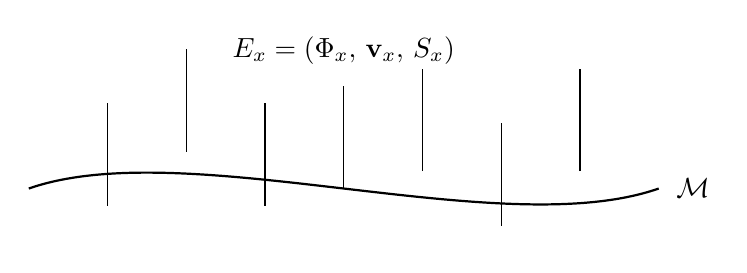
\begin{tikzpicture}
\draw[thick] (-4,0) .. controls (-2,0.7) and (2,-0.7) .. (4,0);
\node[right] at (4.1,0) {$\mathcal{M}$};
\foreach \x/\y in {-3/-0.22,-2/0.47,-1/-0.22,0/0,1/0.22,2/-0.47,3/0.22} {
  \draw (\x,\y) -- ++(0,1.3);
}
\node at (0,1.75) {$E_x = (\Phi_x,\,\mathbf{v}_x,\,S_x)$};
\end{tikzpicture}
\caption{Reputational dynamics as a fiber bundle. Each point $x$ on the interpretive manifold $\mathcal{M}$ carries a fiber of field values $(\Phi,\mathbf{v},S)$. High-curvature zones correspond to regions of rapid narrative divergence.}
\end{figure}

\subsection{Embedding the Visibility Minimization Principle}

The previously defined action functional:
\[
\mathcal{S}_{\text{eff}} = \int \left( L_{\text{task}} - \lambda \Phi - \mu S \right) dt
\]

is now interpreted as a reduced action over the reputational sector of RSVP. Minimizing this action corresponds to selecting trajectories in field space that minimize entropy production while achieving task completion.

\section{A No-Go Theorem for Safe Virality}

We now formalize a fundamental limitation on exposure within the scalar--vector--entropy framework.

\subsection{Preliminaries}

Let $\Phi(x,t)$, $\mathbf{v}(x,t)$, and $S(x,t)$ be the visibility, interpretive flow, and reputational entropy fields defined over a manifold $\mathcal{M}$, with dynamics as previously specified.

Let $P(x,t)$ denote bounded protective capacity:
\[
0 < P(x,t) \leq P_{\max} < \infty
\]

Define \emph{safe operation} as the condition:
\[
S(x,t) \leq P(x,t) \quad \forall x,t
\]

Define \emph{virality} as a regime in which visibility diverges in finite or asymptotically short time:
\[
\int_{\mathcal{M}} \Phi(x,t)\,dx \rightarrow \infty
\]

\subsection{Assumptions}

We require only the following mild conditions:

\medskip
\noindent\textbf{A1 (Entropy Production):}
\[
\frac{\partial S}{\partial t} \geq \alpha |\mathbf{v}|^2 - \beta \mathcal{C}
\quad \text{with } \alpha > 0
\]

\medskip
\noindent\textbf{A2 (Flow Coupling):}
\[
|\mathbf{v}| \geq c_1 |\nabla \Phi|
\]

\medskip
\noindent\textbf{A3 (Nonzero Interaction Density):}
\[
\int_{\mathcal{M}} |\nabla \Phi|^2 dx \rightarrow \infty
\quad \text{as } \Phi \rightarrow \infty
\]

\medskip
\noindent\textbf{A4 (Bounded Correction):}
\[
\mathcal{C}(x,t) \leq C_{\max} < \infty
\]

\medskip

These assumptions encode only that interaction produces distortion, that attention induces flow, and that correction is finite.

\subsection{Main Theorem}

\begin{theorem}[No-Go for Safe Virality]
Under assumptions \emph{A1}--\emph{A4}, there exists no trajectory for which visibility diverges while maintaining safe operation. That is:
\[
\Phi \rightarrow \infty
\quad \Longrightarrow \quad
\exists\, (x,t) \text{ such that } S(x,t) > P(x,t)
\]
\end{theorem}

\begin{proof}
From flow coupling (A2):
\[
|\mathbf{v}|^2 \geq c_1^2 |\nabla \Phi|^2
\]

Substituting into entropy production (A1):
\[
\frac{\partial S}{\partial t}
\geq
\alpha c_1^2 |\nabla \Phi|^2 - \beta C_{\max}
\]

Integrating over $\mathcal{M}$:
\[
\frac{d}{dt} \int_{\mathcal{M}} S\,dx
\geq
\alpha c_1^2 \int_{\mathcal{M}} |\nabla \Phi|^2 dx - \beta C_{\max} |\mathcal{M}|
\]

By assumption A3, as $\Phi \to \infty$:
\[
\int_{\mathcal{M}} |\nabla \Phi|^2 dx \to \infty
\]

Thus:
\[
\frac{d}{dt} \int_{\mathcal{M}} S\,dx \to \infty
\]

which implies $\int_{\mathcal{M}} S\,dx \to \infty$.

Since $P(x,t) \leq P_{\max} < \infty$ by assumption, there must exist a point $(x,t)$ such that:
\[
S(x,t) > P(x,t)
\]

violating safe operation. \hfill$\square$
\end{proof}

\begin{figure}[htbp]
\centering
\begin{tikzpicture}
\draw[->] (0,0) -- (6,0) node[right] {$t$};
\draw[->] (0,0) -- (0,4) node[above] {$\int_{\mathcal{M}} S\,dx$};
\draw[thick] (0,0.4) .. controls (2.5,0.9) and (4,2.8) .. (5.2,4);
\draw[dashed] (0,2.8) -- (5.2,2.8);
\node[left] at (0,2.8) {\small $P_{\max}$};
\draw[dotted] (3.6,0) -- (3.6,2.8);
\node[below] at (3.6,0) {\small $t_c$};
\node at (4.5,3.4) {\small divergence};
\end{tikzpicture}
\caption{No-Go Theorem: as visibility grows, total entropy $\int S\,dx$ diverges and eventually exceeds bounded protective capacity $P_{\max}$ at time $t_c$.}
\end{figure}

\subsection{Corollaries}

\begin{corollary}[Finite Safe Envelope]
For any bounded $P$, there exists a finite upper bound $\Phi_c$ such that $\Phi < \Phi_c$ is required for stability.
\end{corollary}

\begin{corollary}[Superlinear Risk Growth]
Risk grows faster than visibility: $\frac{dR}{d\Phi}$ increases as $\Phi$ increases.
\end{corollary}

\begin{corollary}[Inevitability of Distortion]
No amount of correctness or moral alignment alters the inequality $\frac{dS}{dt} > 0$ under sufficient exposure. The entropy production mechanism is independent of signal quality.
\end{corollary}

\subsection{Interpretation}

The theorem establishes that instability under indiscriminate exposure is not contingent on platform design, cultural factors, or individual behavior. It follows directly from three structural facts: interaction generates entropy, visibility induces interaction, and correction is bounded.

Thus, virality cannot be made safe by better messaging, improved intentions, or adherence to norms. It is constrained by the geometry of the field itself.

\section{Design Implications: Conditions for Safe High Visibility}

The No-Go Theorem for Safe Virality establishes that, under current structural conditions, unbounded visibility is incompatible with bounded protection. This raises a constructive question: what modifications to the underlying field would be required to permit stable high visibility? We treat this as a problem of altering the scalar--vector--entropy dynamics.

\subsection{Necessary Structural Modifications}

To permit regimes in which $\Phi \to \infty$ while maintaining $S(x,t) \leq P(x,t)$, at least one of the following constraints must be violated.

\paragraph{Suppression of Entropy Production.}
If entropy production could be reduced or eliminated ($\alpha \rightarrow 0$), then interpretive activity would no longer generate distortion. However, this would require near-perfect alignment of interpretation across the manifold, implying homogeneity of incentives, beliefs, and interpretive frameworks, which is not observed in open systems.

\paragraph{Unbounded Corrective Capacity.}
Alternatively, one could require $\mathcal{C}(x,t) \rightarrow \infty$, so that all distortions are immediately corrected. This would correspond to universal access to verification, instantaneous propagation of corrections, and perfect trust in correction mechanisms. This condition is incompatible with finite cognitive, institutional, and temporal resources.

\paragraph{Decoupling of Visibility and Interaction.}
If visibility did not induce interaction ($\mathbf{v} \not\sim \nabla \Phi$), then increasing $\Phi$ would not generate interpretive flow. This would require a system in which observation does not entail engagement or reinterpretation---a condition that contradicts the basic structure of communicative systems.

\paragraph{Infinite Protective Capacity.}
Finally, stability could be maintained if $P(x,t) \rightarrow \infty$. This corresponds to agents possessing unlimited legal, institutional, and social defense. Such capacity is restricted to highly resourced entities and cannot be generalized.

\subsection{Conclusion of Impossibility}

Each of the above modifications requires conditions that are physically unrealistic, socially implausible, or structurally incompatible with open systems. Thus, within any finite, heterogeneous, and interactive manifold, safe unbounded visibility remains unattainable.

\subsection{Practical Design Principles}

While safe virality is impossible, systems may be designed to improve stability within bounded regimes.

\paragraph{Gradient Limitation.}
Imposing constraints on $|\nabla \Phi|$ prevents rapid amplification of visibility. This corresponds to rate-limiting dissemination and discouraging sudden global exposure.

\paragraph{Domain Partitioning.}
Structuring the manifold into semi-isolated domains $\mathcal{M} = \bigsqcup_i D_i$ with limited coupling between domains reduces global entropy cascades and localizes distortion.

\paragraph{Entropy-Aware Feedback.}
Exposing agents to estimates of $S(x,t)$ allows adaptive control of exposure $u(t) = f(S, P)$, rather than blind amplification.

\paragraph{Alignment-Weighted Propagation.}
Modifying amplification operators such that $A(x,t) \propto \text{contextual alignment}$ reduces propagation into regions of high interpretive mismatch.

\paragraph{Reputation Buffering Layers.}
Introducing intermediate structures that absorb entropy:
\[
S_{\text{agent}} \ll S_{\text{interface}} \ll S_{\text{global}}
\]
analogous to shock absorbers in dynamical systems.

\section{Asymmetric Vulnerability: Visibility Under Unequal Protective Capacity}

The preceding analysis treats protective capacity $P(x,t)$ as bounded but does not assume it is uniformly distributed. In practice, $P$ varies significantly across agents, and this variation induces a structural asymmetry in exposure dynamics that is independent of any individual's intentions or skill.

Let $P_i \ll P_j$ for agents $i$ and $j$. Then, for identical visibility trajectories $\Phi_i = \Phi_j$, the stability condition $S(x,t) \leq P(x,t)$ is violated earlier for agent $i$ than for agent $j$. There therefore exists a class of agents for whom $\Phi_{c,i} \ll \Phi_{c,j}$: the critical visibility threshold is significantly lower.

Agents with low protective capacity---limited financial resources, absence of institutional affiliation, lack of legal support---enter the unstable regime under levels of exposure that remain safe for highly resourced agents. Thus the same act of publicity produces qualitatively different outcomes depending on $P$.

\subsection{Economic Stratification of the Stability Threshold}

Decompose protective capacity into its constituent components:
\[
P(x,t) = P_{\text{legal}} + P_{\text{institutional}} + P_{\text{network}}
\]

For high-resource agents, $P \gg 1$; for low-resource agents, $P \approx \text{constant (small)}$. Because instability occurs at $\Phi_c$, and $\Phi_c$ depends on $P$, inequality in $P$ produces nonlinear divergence in outcomes:
\[
\Delta P \;\Rightarrow\; \Delta \Phi_c \;\Rightarrow\; \text{phase divergence}
\]

Exposure therefore amplifies pre-existing inequality rather than bypassing it.

\subsection{Narrative Control as Structural Correction}

Agents with high $P$ also possess greater effective corrective capacity. Access to coordinated messaging, media channels, and credibility reinforcement means that for high-resource agents $\mathcal{C} \rightarrow \mathcal{C}_{\text{amplified}}$, while for low-resource agents $\mathcal{C} \approx \text{limited}$, so $\frac{\partial S}{\partial t} \gg 0$ under comparable exposure. The ability to control a narrative is not merely rhetorical skill but a structural extension of $\mathcal{C}$, further widening the gap between agents operating at different levels of $P$.

\subsection{Credentialing as a Stability License}

In many domains, formal credentials function as signals of competence. They also act as proxies for $P$: credentials correlate not only with knowledge but with access to institutional backing, reputational networks, and defensive infrastructure. High-cost credentialing systems impose a barrier ($\text{cost} \uparrow \Rightarrow \text{access} \downarrow$) that selects for agents with higher baseline $P$. Credentials therefore function as stability licenses as much as epistemic certifications---they indicate not only that an agent knows something, but that the agent can safely operate at higher visibility levels without catastrophic exposure to the unstable regime.

\subsection{Inequality as a Field Effect}

The combined effect of unequal $P$, differential correction, and credentialing generates a self-reinforcing loop at the field level. Two agents with identical signals but different $P$ follow distinct trajectories: $(\Phi,S)_i \rightarrow \text{instability}$ while $(\Phi,S)_j \rightarrow \text{stability}$. This divergence is not a one-time event but a dynamic feedback: instability reduces future $P$ (reputational damage limits access to further resources), while stability allows $P$ to grow. The result is:
\[
P_{\text{high}} \uparrow \;\Rightarrow\; \Phi_{c} \uparrow, \qquad P_{\text{low}} \downarrow \;\Rightarrow\; \Phi_{c} \downarrow
\]

Inequality is not external to the visibility system; it is generated and amplified by the same scalar--vector--entropy dynamics.

\begin{figure}[htbp]
\centering
\begin{tikzpicture}
\draw[->] (0,0) -- (7,0) node[right] {$\Phi$};
\draw[->] (0,0) -- (0,4.5) node[above] {$S$};
% low-P agent
\draw[thick] (0,0.3) .. controls (2,1.2) and (3.2,3.2) .. (4,4.3);
\draw[dashed] (0,1.5) -- (6.5,1.5);
\node[left] at (0,1.5) {\small $P_i$};
\draw[dotted] (2.35,0) -- (2.35,1.5);
\node[below] at (2.35,0) {\small $\Phi_{c,i}$};
% high-P agent
\draw[thick,gray!70] (0,0.3) .. controls (2,1.2) and (3.2,3.2) .. (4,4.3);
\draw[dashed,gray!60] (0,3.2) -- (6.5,3.2);
\node[left] at (0,3.2) {\small $P_j$};
\draw[dotted,gray!60] (4.7,0) -- (4.7,3.2);
\node[below] at (4.7,0) {\small $\Phi_{c,j}$};
% labels
\node[right] at (4.1,4.1) {\small same entropy trajectory};
\draw[<->] (5.5,1.5) -- (5.5,3.2);
\node[right] at (5.55,2.35) {\small $\Delta P$};
\end{tikzpicture}
\caption{Unequal critical visibility thresholds under identical entropy trajectories. Both agents follow the same entropy curve, but agent $i$ (lower $P_i$) crosses into instability at $\Phi_{c,i}$, while agent $j$ remains stable until $\Phi_{c,j} \gg \Phi_{c,i}$. The same field acts on both; the instability boundary is not located at the same place.}
\end{figure}

\section{An Inequality Amplification Theorem}

We now formalize the claim that unequal protective capacity produces unequal exposure outcomes even under identical visibility trajectories.

\subsection{Setup}

Let two agents $i$ and $j$ evolve on the same interpretive manifold under identical visibility input:
\[
\Phi_i(t) = \Phi_j(t) = \Phi(t)
\]
and suppose their entropy dynamics satisfy
\[
\frac{dS_k}{dt} = \alpha_k |\mathbf{v}_k|^2 - \beta_k \mathcal{C}_k,
\qquad k \in \{i,j\}.
\]

Let protective capacity be bounded and unequal:
\[
0 < P_i < P_j < \infty.
\]

Define the instability time
\[
\tau_k = \inf \{ t > 0 : S_k(t) > P_k \}.
\]

\begin{theorem}[Inequality Amplification Under Equal Exposure]
Assume that agents $i$ and $j$ are subject to the same visibility trajectory $\Phi(t)$, with comparable flow coupling
\[
|\mathbf{v}_i| \asymp |\mathbf{v}_j| \asymp |\nabla \Phi|,
\]
and that their corrective capacities satisfy
\[
\mathcal{C}_i \leq \mathcal{C}_j.
\]
If $P_i < P_j$, then the lower-capacity agent becomes unstable no later than the higher-capacity agent:
\[
\tau_i \leq \tau_j.
\]
Moreover, if either $P_i \ll P_j$ or $\mathcal{C}_i \ll \mathcal{C}_j$, then generically
\[
\tau_i \ll \tau_j.
\]
\end{theorem}

\begin{proof}
Because the visibility trajectory is identical, both agents are driven by the same exposure field $\Phi(t)$. By the flow-coupling assumption,
\[
|\mathbf{v}_i|^2 \asymp |\mathbf{v}_j|^2 \asymp |\nabla \Phi|^2.
\]
Thus entropy production is of the same order for both agents, while the corrective term is weaker for agent $i$:
\[
\beta_i \mathcal{C}_i \leq \beta_j \mathcal{C}_j
\]
under comparable coefficients. Hence, for equal initial conditions $S_i(0)=S_j(0)$, agent $i$ accumulates entropy at least as rapidly relative to available protection. Since instability occurs when $S_k(t) > P_k$, and since $P_i < P_j$, agent $i$ reaches the instability boundary no later than agent $j$, giving $\tau_i \leq \tau_j$. If the asymmetry is large, the crossing times separate accordingly, giving $\tau_i \ll \tau_j$. \hfill$\square$
\end{proof}

\begin{corollary}[Unequal Critical Visibility Thresholds]
Under the same assumptions, the critical visibility thresholds satisfy
\[
\Phi_{c,i} \leq \Phi_{c,j},
\]
with $\Phi_{c,i} \ll \Phi_{c,j}$ when the asymmetry in protection or correction is sufficiently large.
\end{corollary}

\begin{proof}
The critical threshold is defined by $S_k(\Phi_{c,k}) = P_k$. Since agent $i$ has lower protection and no greater corrective capacity, this equality is reached at a lower visibility level. \hfill$\square$
\end{proof}

The theorem shows that exposure does not merely reveal pre-existing inequality; it amplifies it dynamically. Agents with lower protective capacity do not simply face somewhat greater risk---they cross into instability earlier, at lower visibility, and with less ability to recover:
\[
P_{\text{low}} \;\Rightarrow\; \Phi_c \downarrow \;\Rightarrow\; \tau \downarrow \;\Rightarrow\; S \uparrow.
\]

\section{A Selection Bias Theorem for Observed Visibility Success}

The unequal danger of exposure is further obscured by a sampling effect. Public discourse does not observe all trajectories equally; it preferentially observes those that remain visible after exposure. This induces a survivor bias that makes publicity appear safer and more meritocratic than it is across the full population.

\subsection{Setup}

Let each agent $k$ have visibility trajectory $\Phi_k(t)$, entropy trajectory $S_k(t)$, and protective capacity $P_k(t)$. Define the survival indicator
\[
\mathbf{1}_{\mathrm{surv},k}(t)
=
\begin{cases}
1 & \text{if } S_k(t) \leq P_k(t),\\
0 & \text{if } S_k(t) > P_k(t),
\end{cases}
\]
and the visible sample $\mathcal{V}(t)=\{k : \mathbf{1}_{\mathrm{surv},k}(t)=1\}$. Let $Y_k(t)$ measure some outcome (reach, influence, continued credibility). The true expected outcome across all exposed agents is $\mathbb{E}[Y(t)]$; the observed expected outcome among survivors is $\mathbb{E}[Y(t)\mid k\in \mathcal{V}(t)]$.

\begin{theorem}[Selection Bias in Observed Visibility Success]
Suppose that instability removes or attenuates agents from the visible sample ($S_k(t) > P_k(t) \Rightarrow k \notin \mathcal{V}(t)$ or $Y_k(t)$ becomes unobservable), lower protective capacity increases the probability of instability under exposure, and survival is positively correlated with observed success. Then:
\[
\mathbb{E}[Y(t)\mid k\in \mathcal{V}(t)] \geq \mathbb{E}[Y(t)],
\]
with strict inequality whenever instability removes a nonzero mass of low-protection trajectories from observation.
\end{theorem}

\begin{proof}
By construction, the visible sample conditions on survival: $k\in \mathcal{V}(t) \iff S_k(t)\leq P_k(t)$. Agents whose entropy exceeds protection are removed from view, suppressed, discredited, or no longer legible as successful cases. The removed subset is disproportionately composed of low-$P$ agents. Since survival is positively correlated with continued visibility and measurable success, conditioning on $k\in \mathcal{V}(t)$ biases the sample upward. If a positive-measure set of low-$P$ agents contributes lower values of $Y_k(t)$ than the surviving set, the inequality is strict. \hfill$\square$
\end{proof}

\begin{corollary}[Underestimation of Exposure Risk]
If observers estimate the safety of publicity from the visible sample alone, they will systematically underestimate the true risk of exposure:
\[
\mathbb{E}[\emph{risk} \mid k\in \mathcal{V}(t)] < \mathbb{E}[\emph{risk}].
\]
\end{corollary}

\begin{corollary}[Class Skew in the Visible Sample]
If protective capacity $P$ is positively correlated with wealth, institutional affiliation, or credentialed status, then the visible survivor set $\mathcal{V}(t)$ is biased toward such agents.
\end{corollary}

The two corollaries together explain why publicity culture simultaneously appears meritocratic and is not. The first corollary shows that observers underestimate how dangerous exposure is across the full population. The second shows that who remains visible is systematically skewed toward those with prior structural advantages. Both effects follow from the same sampling mechanism, not from any conspiracy of misrepresentation.

In this sense, the ideology of indiscriminate publicity is sustained by an observational artifact:
\[
\text{visible success} \neq \text{typical outcome under exposure}.
\]

The apparent safety of visibility is an illusion generated by the disappearance of its casualties. Those who are destabilized by exposure exit the visible field precisely because they were destabilized, leaving behind a survivor population that looks as though exposure were uniformly beneficial.

\section{AGI as an Attempted Violation of the No-Go Theorem}

The vision of a decentralized society of AGI minds may be interpreted as an attempt to construct a system in which the conditions of the No-Go Theorem for Safe Virality are no longer satisfied. Specifically, such a system seeks to reduce entropy production during interaction, increase corrective capacity through distributed cognition, and redistribute exposure across a network rather than concentrating it on individuals. We analyze these modifications in the language of scalar--vector--entropy dynamics.

\subsection{Modified Entropy Equation}

In the AGI regime, the entropy equation becomes:
\[
\frac{\partial S}{\partial t}
=
\alpha_{\text{AGI}} |\mathbf{v}|^2
-
\beta_{\text{AGI}} \mathcal{C}_{\text{net}}
\]

with $\alpha_{\text{AGI}} \ll \alpha_{\text{human}}$ (improved interpretive alignment) and $\mathcal{C}_{\text{net}} \gg \mathcal{C}_{\text{individual}}$ (distributed correction).

The viability of the system depends on whether:
\[
\beta_{\text{AGI}} \mathcal{C}_{\text{net}} \geq \alpha_{\text{AGI}} |\mathbf{v}|^2
\]
can be maintained under increasing $\Phi$. This is not a guaranteed outcome of decentralization, but a structural requirement that any proposed AGI architecture must satisfy if it is to constitute a genuine escape from the constraints previously derived.

\section{Escape Conditions for Stable High Visibility}

\subsection{AGI Stability Inequality}

Define the stability condition $\frac{dS}{dt} \leq 0$. Substituting and using flow coupling $|\mathbf{v}| \sim |\nabla \Phi|$, we obtain:
\[
\alpha |\nabla \Phi|^2 \leq \beta \mathcal{C}
\]

Thus, stable high visibility requires:
\[
|\nabla \Phi|^2 \leq \frac{\beta}{\alpha} \mathcal{C}
\]

This inequality shows that stability depends not on absolute visibility, but on the ratio $\mathcal{C}/\alpha$: correction capacity per unit of entropy production. AGI systems attempt to increase this ratio dramatically, but the requirement follows the same structure as in human systems. The escape is conditional, not categorical.

\section{The Re-Emergence Theorem for Distributed Systems}

Even if instability is suppressed locally, it may reappear at the global level.

\begin{theorem}[Re-Emergence of Entropy]
Let the system consist of domains $D_i$, each satisfying $\frac{dS_i}{dt} \leq 0$. Suppose interactions between domains introduce representational mismatch:
\[
\Delta_{ij} = \|\emph{representation}_i - \emph{representation}_j\| > 0
\]
Then global entropy satisfies:
\[
\frac{dS_{\emph{global}}}{dt}
\geq
\sum_{i,j} \gamma \Delta_{ij} |\mathbf{v}_{ij}|
\]
for some $\gamma > 0$.
\end{theorem}

\begin{proof}
Each interface between domains $D_i$ and $D_j$ carries a flow $\mathbf{v}_{ij}$ driven by the visibility gradient across the boundary. Where $\Delta_{ij} > 0$, the interpretive states are mismatched, and each unit of cross-domain flow generates entropy proportional to the mismatch. Summing over all interfaces yields the stated bound. \hfill$\square$
\end{proof}

The conclusion is immediate: local stability does not imply global stability. Entropy re-emerges at the boundaries of interpretation, which is precisely where domains with different priors, objectives, or representational structures come into contact.

\begin{figure}[htbp]
\centering
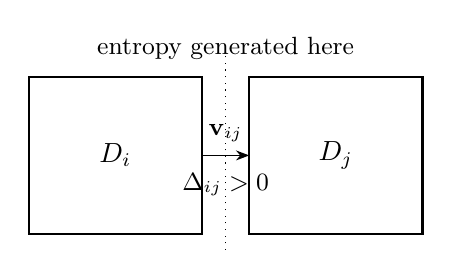
\begin{tikzpicture}[>=Stealth]
\draw[thick] (0,0) rectangle (2.2,2);
\draw[thick] (2.8,0) rectangle (5.0,2);
\node at (1.1,1) {$D_i$};
\node at (3.9,1) {$D_j$};
\draw[->] (2.2,1) -- (2.8,1);
\node[above] at (2.5,1.05) {\small $\mathbf{v}_{ij}$};
\node[below] at (2.5,0.9) {\small $\Delta_{ij}>0$};
\node[above] at (2.5,2.1) {\small entropy generated here};
\draw[dotted] (2.5,-0.2) -- (2.5,2.3);
\end{tikzpicture}
\caption{Re-Emergence Theorem: even when each domain $D_i$ is locally stable, cross-domain flow across a representational mismatch $\Delta_{ij}>0$ generates global entropy at their interface.}
\end{figure}

\subsection{Distributed Visibility and Load Redistribution}

In AGI systems, the unit of exposure shifts from individual agents to networked processes. Let visibility be distributed:
\[
\Phi = \sum_i \Phi_i
\]
with each node carrying a fraction. Then local entropy satisfies $S_i \sim f(\Phi_i)$, and if $\Phi_i \ll \Phi_{\text{global}}$, then $S_i \ll S_{\text{individual}}$.

However, this produces load redistribution rather than load elimination. The system reduces risk per node by distributing exposure, but:
\[
\sum_i S_i \rightarrow S_{\text{global}} \uparrow
\]

Entropy is not eliminated but displaced, producing local stability alongside global complexity and potentially hidden instabilities at the level of the aggregate.

\section{Resonance as Entropy Suppression}

Goertzel's notion of distributed resonance may be interpreted formally as a mechanism for reducing entropy production. Resonance corresponds to alignment of interpretive states across agents:
\[
\mathbf{v}_i \approx \mathbf{v}_j \quad \Rightarrow \quad \Delta_{ij} \rightarrow 0
\]

Under this condition, entropy production becomes:
\[
\frac{dS}{dt} \sim \alpha \sum_{i,j} \Delta_{ij}^2 \rightarrow 0
\]

This is the strongest possible suppression mechanism and represents a genuine modification of the field parameters. However, perfect resonance requires shared representations, aligned objectives, and low noise across the entire manifold. Any deviation reintroduces entropy growth, making resonance a sufficient but fragile condition.

\subsection{Adversarial Dynamics in Post-Human Systems}

Even in AGI ecologies, adversarial dynamics may persist. Sources of reintroduced entropy include competing optimization targets, resource constraints, representational incompatibility, and evolutionary pressure among subsystems. The vector field decomposes as:
\[
\mathbf{v} = \mathbf{v}_{\text{coherent}} + \mathbf{v}_{\text{adversarial}}
\]
with $\mathbf{v}_{\text{adversarial}} \sim \nabla \Delta$, driven by gradients in representational mismatch. Unless adversarial components are actively suppressed, $\frac{dS}{dt} > 0$ reasserts itself, and instability reappears. The transition to AGI does not by itself eliminate competitive incentives; it shifts the substrate on which they operate.

\section{AGI as Field Engineering}

The transition described by Goertzel may be understood precisely as an attempt to engineer the underlying field parameters:
\[
\alpha \downarrow, \quad \beta \uparrow, \quad P \uparrow
\]

so that $\alpha |\mathbf{v}|^2 \leq \beta \mathcal{C}$ holds under arbitrarily large $\Phi$. This framing is precise and non-trivial. AGI is not merely intelligence amplification but modification of the thermodynamics of interpretation: an attempt to change the coupling constants of the social field rather than to operate more skillfully within them.

Whether this engineering is achievable, stable under perturbation, and globally rather than locally effective remains the central open question. The RSVP framework does not resolve it, but it specifies exactly what would have to be true for the answer to be yes.

\section{Phase Structure of Visibility--Entropy Systems}

We now classify regimes of visibility and reputational dynamics as phases of a non-equilibrium system.

\subsection{Order Parameters}

Define the following dimensionless quantities:
\[
\kappa = \frac{\beta \mathcal{C}}{\alpha |\nabla \Phi|^2}
\quad \text{(stability ratio)}
\]
\[
\eta = \frac{|\mathbf{v}_{\text{adversarial}}|}{|\mathbf{v}|}
\quad \text{(adversarial fraction)}
\]
\[
\chi = \mathrm{Var}(\text{representations})
\quad \text{(interpretive heterogeneity)}
\]

The three conditions $\kappa > 1$, $\eta \approx 0$, and $\chi \approx 0$ jointly define a stable, coherent, high-fidelity signaling regime. The conditions $\kappa < 1$, $\eta \rightarrow 1$, and $\chi \gg 1$ jointly define instability.

\subsection{Four Phases}

\paragraph{Phase I: Low-Visibility Coherent Regime.}
$\Phi$ small, $\kappa \gg 1$, $\eta \approx 0$. Characteristics: high signal integrity, low entropy production, stable local interactions. This corresponds to small communities, private work, or tightly aligned domains.

\paragraph{Phase II: Competitive Visibility Regime.}
$\Phi$ increasing, $\kappa \sim 1$, $\eta > 0$. Characteristics: relative evaluation (ranking, markets), emergence of adversarial flows, increasing entropy. This includes competitive classrooms, markets, and early-stage publicity.

\paragraph{Phase III: Turbulent Virality Regime.}
$\Phi \gg 1$, $\kappa \ll 1$, $\eta \approx 1$. Characteristics: runaway entropy production, narrative fragmentation, reputational instability. This is the regime of indiscriminate virality.

\paragraph{Phase IV: Resonant Distributed Regime (Hypothesized).}
$\Phi \gg 1$, $\kappa \gg 1$, $\eta \approx 0$. Characteristics: high visibility with low entropy, distributed correction, alignment across agents. This corresponds to the AGI resonance scenario. It is the only phase in which the No-Go Theorem's assumptions are violated, and its accessibility from Phase II without passing through Phase III is the central open question.

\begin{figure}[htbp]
\centering
\begin{tikzpicture}[scale=1.05]
\draw[->] (0,0) -- (7,0) node[right] {$\Phi$ (visibility)};
\draw[->] (0,0) -- (0,6) node[above] {$\kappa$ (stability)};
\draw[dashed] (0,3) -- (7,3);
\node[left] at (0,3) {$\kappa=1$};
\node at (1.4,5.0) {\small \textbf{I}};
\node at (3.2,4.3) {\small \textbf{II}};
\node at (5.6,1.8) {\small \textbf{III}};
\node at (5.6,5.0) {\small \textbf{IV}};
% Human trajectory I → III
\draw[thick,->] (1.2,4.8) .. controls (3,4.2) and (4.2,3.2) .. (5.5,1.7);
\node[below right] at (3.5,3.5) {\small human};
% AGI trajectory II → IV
\draw[thick,->,dashed] (3.2,4.1) .. controls (4.5,4.6) and (5.2,4.8) .. (5.8,5.1);
\node[above] at (4.5,4.75) {\small AGI attempt};
\end{tikzpicture}
\caption{Master phase diagram. The dashed horizontal line marks $\kappa=1$, the stability boundary. Human systems typically flow from coherent (I) through competitive (II) into turbulent virality (III). The AGI vision attempts a direct transition from II to the resonant regime (IV), bypassing instability—a path whose viability is the central open problem of the theory.}
\end{figure}

\subsection{Phase Transitions and Hysteresis}

Define $\Phi_c$ such that $\kappa(\Phi_c) = 1$. Crossing this threshold induces a transition from Phase II to Phase III. Near the critical point, entropy production scales as:
\[
\frac{dS}{dt} \sim (\Phi - \Phi_c)^\gamma
\]
for some $\gamma > 0$, producing rapid escalation of instability. Critically, once in Phase III, the transition is not easily reversed. Returning to stability requires substantial reduction of $\Phi$ or a significant increase in $\mathcal{C}$, and the system exhibits hysteresis: the history of high visibility leaves a residue that makes subsequent instability easier to trigger.

\begin{figure}[htbp]
\centering
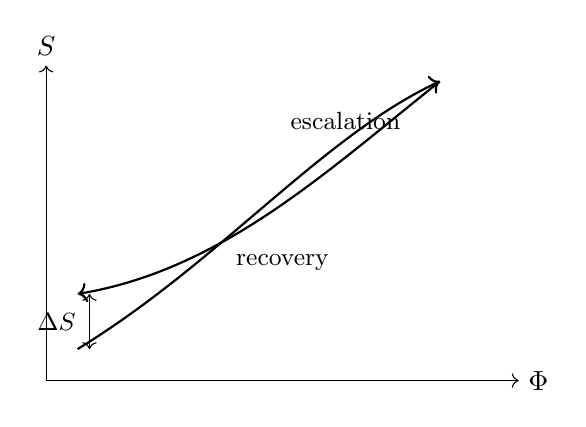
\begin{tikzpicture}
\draw[->] (0,0) -- (6,0) node[right] {$\Phi$};
\draw[->] (0,0) -- (0,4) node[above] {$S$};
\draw[thick,->] (0.4,0.4) .. controls (2.2,1.5) and (3.5,3.1) .. (5,3.8);
\draw[thick,->] (5,3.8) .. controls (3.5,2.6) and (2.2,1.4) .. (0.4,1.1);
\node at (3.8,3.3) {\small escalation};
\node at (3.0,1.5) {\small recovery};
\draw[<->] (0.55,0.4) -- (0.55,1.1);
\node[left] at (0.5,0.75) {\small $\Delta S$};
\end{tikzpicture}
\caption{Hysteresis in visibility--entropy dynamics. The escalation path (upper curve) and the recovery path (lower curve) do not coincide. Residual entropy $\Delta S > 0$ persists after visibility is reduced, encoding the irreversibility of reputational damage.}
\end{figure}

\subsection{Phase IV Accessibility and Failure Modes}

AGI systems attempt to transition directly from Phase II to Phase IV, bypassing turbulence. This requires simultaneously achieving $\kappa \gg 1$, $\eta \rightarrow 0$, and $\chi \rightarrow 0$ under large $\Phi$. Even if Phase IV is reached locally, characteristic failure modes include interface instability (entropy generated at domain boundaries where $\chi_{ij} > 0$), adversarial phase nucleation (small adversarial regions expanding, analogous to nucleation in physical phase transitions), and correction saturation (when $\mathcal{C}_{\text{net}}$ reaches its capacity limit, $\kappa$ falls and the system re-enters Phase III). Phase IV is therefore metastable rather than unconditionally stable.

\section{Empirical Signatures of Visibility--Entropy Dynamics}

To render the theory testable, we introduce observable quantities corresponding to the scalar--vector--entropy fields.

\subsection{Observable Proxies}

Let $\hat{\Phi}(t)$ denote measured attention (views, reach, mentions), $\hat{\mathbf{v}}(t)$ interaction flow (shares, replies, citations), $\hat{S}(t)$ a distortion proxy (narrative variance, contradiction density, rumor proliferation rate), and $\hat{\mathcal{C}}(t)$ correction capacity (fact-checking frequency, authoritative response rate). From these, define:
\[
\hat{\kappa}(t) = \frac{\hat{\mathcal{C}}}{\mathrm{Var}(\hat{\mathbf{v}})},
\quad
\hat{\eta}(t) = \frac{\text{adversarial interactions}}{\text{total interactions}},
\quad
\hat{\chi}(t) = \text{variance of interpretations}
\]

These are imperfect but measurable proxies for the underlying field parameters.

\subsection{Early Warning Signals of Instability}

As systems approach the critical threshold $\Phi_c$, characteristic signals emerge prior to full transition. These include variance inflation in $\hat{S}$ (increasing disagreement, multiple competing narratives), breakdown of correlation between content and interpretation (semantic drift), compression of reaction time (faster responses with less verification, increasing entropy production rate), and growth of $\hat{\eta}$ (adversarial flow becoming a larger fraction of total interaction).

These signals are the field-theoretic analogues of critical slowing down and fluctuation growth observed near phase transitions in physical systems.

\subsection{Signatures of the Turbulent Virality Regime}

Once $\Phi > \Phi_c$, the system enters Phase III. Observable signatures include superlinear growth of distortion ($\hat{S}(t) \sim \hat{\Phi}(t)^\gamma$ with $\gamma > 1$), narrative fragmentation ($\hat{\chi} \gg 1$, with multiple incompatible interpretations coexisting), persistence of false signals after correction events ($\hat{S}$ fails to return to baseline following authoritative correction), and decoupling of truth and reach ($\mathrm{Corr}(\text{accuracy}, \hat{\Phi}) \rightarrow 0$, so visibility no longer tracks correctness).

\subsection{Recovery and Hysteresis Signatures}

After instability, recovery is slow and incomplete. Observable signatures include delayed decay of $\hat{S}$ even after $\hat{\Phi}$ is reduced, residual distortion above the pre-exposure baseline ($\hat{S}_{\text{final}} > \hat{S}_{\text{initial}}$), and rapid re-entry into Phase III upon subsequent increases in visibility. This pattern is the empirical signature of the irreversibility predicted by the entropy production model.

\subsection{Empirical Tests of the AGI Resonance Hypothesis}

An AGI system that genuinely achieves Phase IV would need to demonstrate stable high $\hat{\Phi}$, bounded or decreasing $\hat{S}$, low $\hat{\eta}$, and low $\hat{\chi}$ across domain boundaries—formally:
\[
\frac{d\hat{S}}{dt} \leq 0 \quad \text{as } \hat{\Phi} \rightarrow \infty
\]

The theory predicts failure if $\hat{S}$ or $\hat{\eta}$ increase with $\hat{\Phi}$, indicating that the system has not escaped the entropy constraints but merely redistributed them to a scale not yet observed. This is a falsifiable prediction that can be applied to real decentralized AI systems as they are developed and deployed.

\subsection{Falsifiability and Theoretical Limits}

The theory is falsified if a system demonstrates $\Phi \rightarrow \infty$ while $S \rightarrow 0$ without centralized control or trivial homogeneity. Such a system would violate the entropy production assumption at the core of the framework. Candidate test environments include large-scale decentralized AI systems, collaborative knowledge networks operating at scale, and hybrid human-AI communication infrastructure. The theory does not predict that such systems cannot exist, but that if they exist and remain stable, they must have achieved a genuine modification of field parameters---a change in the thermodynamics of interpretation rather than a more efficient operation within the existing regime.

\begin{figure}[htbp]
\centering
\begin{tikzpicture}[>=Stealth,node distance=0pt]
\node (local)  at (0,0)   {$D_i$};
\node (global) at (4.5,0) {$\mathcal{M}$};
\node (S)      at (2.25,-2.2) {$S$};
\draw[->] (local)  -- (global) node[midway,above] {$\iota$};
\draw[->] (global) -- (S)      node[midway,right] {$\mathcal{E}$};
\draw[->] (local)  -- (S)      node[midway,left]  {$\mathcal{E}_i$};
\node at (2.25,-0.7) {\small $\not\circlearrowleft$};
\end{tikzpicture}
\caption{Non-commutativity as entropy. When the local entropy $\mathcal{E}_i$ and the restriction of global entropy $\mathcal{E}$ do not agree---i.e., when the diagram fails to commute---the mismatch constitutes entropy production at the domain boundary. Entropy is the measure of categorical failure.}
\end{figure}

\clearpage
\section{Coherence Thermodynamics as a Semantic Sector of RSVP}

We now integrate Coherence Thermodynamics (CT)~\cite{barton2025} into the scalar--vector--entropy framework, treating reputational dynamics as a thermodynamic sector of the field theory developed above. This establishes a direct correspondence between visibility-driven interaction and non-equilibrium semantic thermodynamics, moving the relationship from analogy to structural identification.

\subsection{Field Identification}

We identify the CT variables with the field-theoretic quantities already defined:
\[
S(x,t) = \int w(x)\, S^*(x,t)\,dx,
\qquad
\mathbf{v}(x,t) \sim j_R(x,t),
\qquad
T^*(x,t) \sim f(|\nabla \Phi(x,t)|).
\]

Here $S^*$ denotes local contradiction load in the CT sense, and reputational entropy $S$ is its coarse-grained projection over the interpretive manifold. Interpretive flow $\mathbf{v}$ corresponds to the coherence flux $j_R$, while visibility gradients act as sources of semantic temperature. The identification is not merely formal: the CT entropy balance equation
\[
\frac{\partial s}{\partial t} = -\nabla \cdot j_R + \sigma
\]
maps directly onto the RSVP entropy equation with advective, diffusive, and production terms.

\subsection{Visibility-Induced Semantic Heating}

\begin{theorem}[Visibility-Induced Semantic Heating]
Increases in visibility gradients induce increases in semantic temperature and therefore increase semantic entropy production:
\[
|\nabla \Phi| \uparrow \quad \Rightarrow \quad T^* \uparrow \quad \Rightarrow \quad \frac{\partial S}{\partial t} \uparrow.
\]
\end{theorem}

\begin{proof}
By field coupling, interpretive flow satisfies $\mathbf{v} \sim \nabla \Phi$. Entropy production scales as $\alpha|\mathbf{v}|^2$, while CT defines semantic temperature as the degree of agitation in interpretive phase. Increasing $|\nabla \Phi|$ increases both $|\mathbf{v}|^2$ and $T^*$, driving increased entropy production. \hfill$\square$
\end{proof}

\subsection{Virality as a High-Temperature Phase}

Using the CT coherence functional
\[
C_T = \frac{1}{T^* S^*},
\]
the instability condition acquires a thermodynamic form:
\[
\text{Virality} \;\Rightarrow\; T^* \uparrow \;\Rightarrow\; S^* \uparrow \;\Rightarrow\; C_T \downarrow.
\]

The transition from controlled dissemination to virality corresponds to a phase transition from a low-temperature coherent regime to a high-temperature incoherent one. The No-Go Theorem becomes a statement about unavoidable coherence collapse under unbounded semantic heating. This thermodynamic interpretation allows the result to be understood not only as a structural limitation, but as a direct consequence of coherence collapse under semantic heating.

\begin{figure}[htbp]
\centering
\begin{tikzpicture}[scale=1.2]
\draw[->] (0,0) -- (5.5,0) node[right] {$T^*$};
\draw[->] (0,0) -- (0,5.5) node[above] {$C_T$};
\draw[thick] (0.4,5) .. controls (1.5,3.5) and (3,1.8) .. (5,0.5);
\node at (1.0,4.5) {\small Coherent};
\node at (2.8,2.8) {\small Competitive};
\node at (4.3,1.1) {\small Turbulent};
\draw[dotted] (1.8,0) -- (1.8,3.0);
\node[below] at (1.8,0) {\small $T^*_c$};
\end{tikzpicture}
\caption{Coherence $C_T$ decreases as semantic temperature $T^*$ increases. The dotted line marks the critical temperature $T^*_c$ above which the turbulent virality regime is entered. The four phases of the earlier diagram correspond to positions along this curve.}
\end{figure}

\subsection{Entropy Export and Manifold Redistribution}

In CT, local order is achieved by exporting contradiction:
\[
\frac{\partial s}{\partial t} = -\nabla \cdot j_R + \sigma.
\]

Within the field framework, exported entropy is not removed from the system but redistributed across the manifold:
\[
S_{\text{local}} \downarrow \quad \Longrightarrow \quad S_{\text{global}} \uparrow.
\]

Viral events therefore act as entropy sources for surrounding domains, producing destabilization that propagates beyond the originating system. This explains the observed diffusion of controversy and narrative fragmentation into adjacent communities that had no direct contact with the original exposure event.

\subsection{The Filtering Condition as Boundary Constraint}

The CT principle governing what enters a system --- that inputs should not exceed an entropic threshold --- corresponds within the field framework to a boundary condition:
\[
\Phi(x,t) = 0 \quad \text{for regions where } S^*_{\text{input}} > S^*_{\text{threshold}}.
\]

Selective dissemination is therefore not merely a practical heuristic but the correct entropy-filtering boundary condition. Instability arises when this condition fails and high-entropy inputs penetrate the system, overwhelming its corrective capacity.

\subsection{AGI as a Low-Temperature Limit}

The hypothesized Phase IV corresponds to the CT limit:
\[
T^* \to 0, \quad S^* \to S_0, \quad C_T \to \infty.
\]

This requires that entropy production never exceeds export:
\[
\sigma \leq \nabla \cdot j_R \quad \forall x,t.
\]

Any residual mismatch between domains produces $\Delta_{ij} > 0$ and therefore $\frac{dS}{dt} > 0$, reintroducing entropy through boundary interactions, consistent with the Re-emergence Theorem.

\subsection{Socio-Economic Interpretation}

The thermodynamic structure clarifies the inequality results. High-resource agents effectively operate in low-temperature, high-coherence regimes ($T^* \downarrow$, $C_T \uparrow$), while low-resource agents operate in high-temperature regimes ($T^* \uparrow$, $C_T \downarrow$). Economic inequality therefore corresponds to differential access to low-entropy regions of the interpretive manifold. Credentialing systems function not only as epistemic filters but as mechanisms granting access to protected low-temperature zones with reduced entropy production per interaction.

\section{A Variational Formulation for the Unified Semantic Field Theory}

We now propose a minimal Lagrangian density whose Euler--Lagrange structure reproduces the coupled dynamics of visibility, contradiction, and coherence. The purpose is not to claim a final microscopic derivation, but to provide a consistent variational scaffold unifying the local thermodynamic laws of CT with the global transport geometry of the field framework.

\subsection{Dynamical Variables}

Let the dynamical fields on $\mathcal{M}$ be $\Phi(x,t)$ (visibility potential), $\phi(x,t)$ (semantic phase), $S(x,t)$ (coarse-grained contradiction entropy), and $\mathbf{v}(x,t)$ (interpretive transport). We treat the CT coherence scalar $\alpha$ as derived from $(\phi, S)$, and semantic temperature $T^*$ as derived from phase agitation and visibility forcing:
\[
T^* = T_0 + \gamma(\partial_t \phi)^2 + \gamma_\Phi |\nabla \Phi|^2 + \gamma_S S.
\]

This identifies three sources of semantic heating: phase fluctuation, visibility gradient, and accumulated contradiction.

\subsection{Minimal Lagrangian Density}

We propose the effective Lagrangian density:
\[
\mathcal{L}
=
\frac{a}{2}(\partial_t \phi)^2
-
\frac{b}{2}|\nabla \phi|^2
+
\frac{c}{2}|\mathbf{v}|^2
-
U(\Phi)
-
W(S)
-
\lambda S |\nabla \phi|^2
-
\mu \,\mathbf{v}\cdot \nabla \Phi
-
\nu \,\mathbf{v}\cdot \nabla S
-
\xi \,\Phi S.
\]

The phase kinetic term $\frac{a}{2}(\partial_t \phi)^2$ encodes semantic agitation, providing the basis for semantic temperature. The gradient term $-\frac{b}{2}|\nabla \phi|^2$ penalizes incoherent phase deformation, acting as coherence elasticity. The transport energy $\frac{c}{2}|\mathbf{v}|^2$ represents the energetic cost of interpretive flow. The coupling $-\lambda S|\nabla \phi|^2$ states that contradiction load amplifies the cost of maintaining coherent phase structure. The transport couplings $-\mu\,\mathbf{v}\cdot\nabla\Phi$ and $-\nu\,\mathbf{v}\cdot\nabla S$ encode the core principle that flow is driven by gradients in visibility and entropy. Finally, $-\xi\,\Phi S$ states that visibility and contradiction mutually reinforce under exposure.

\subsection{Euler--Lagrange Consequences}

Variation with respect to $\mathbf{v}$ gives:
\[
\mathbf{v} = \frac{\mu}{c}\nabla \Phi + \frac{\nu}{c}\nabla S,
\]
reproducing the RSVP principle that interpretive flow is driven by visibility and contradiction gradients. Variation with respect to $\phi$ gives:
\[
a\,\partial_t^2 \phi - b\,\Delta \phi - \lambda \nabla\cdot(S \nabla \phi)=0,
\]
describing a phase field whose coherence is destabilized by contradiction load. Variation with respect to $\Phi$ and $S$ respectively yield forcing and contradiction balance equations coupling all fields together.

\subsection{Dissipative Entropy Balance}

Because CT includes irreversible entropy production and export, the Lagrangian must be supplemented with a dissipative balance:
\[
\frac{\partial S}{\partial t}
+
\nabla\cdot(S\mathbf{v})
=
D_S \Delta S
+
\alpha |\mathbf{v}|^2
+
\alpha_\phi |\nabla \phi|^2
-
\beta \mathcal{C},
\qquad \sigma \geq 0.
\]

This is the unified non-equilibrium law combining advection, diffusion, production from interpretive activity and phase strain, and correction.

\subsection{Coherence Functional and Master Inequality}

Adopting the CT coherence form $C_T = 1/(T^* S)$, the causal chain becomes:
\[
\Phi \uparrow \;\Rightarrow\; |\nabla \Phi| \uparrow \;\Rightarrow\; T^* \uparrow \;\Rightarrow\; S \uparrow \;\Rightarrow\; C_T \downarrow.
\]

\begin{figure}[htbp]
\centering
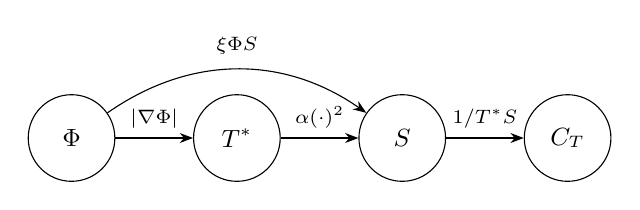
\begin{tikzpicture}[node distance=2.1cm, >=Stealth]
\node[draw,circle,minimum size=1.1cm,align=center,font=\small] (phi)  {$\Phi$};
\node[draw,circle,minimum size=1.1cm,align=center,font=\small] (temp) [right of=phi]  {$T^*$};
\node[draw,circle,minimum size=1.1cm,align=center,font=\small] (S)    [right of=temp] {$S$};
\node[draw,circle,minimum size=1.1cm,align=center,font=\small] (CT)   [right of=S]    {$C_T$};
\draw[->] (phi)  -- (temp) node[midway,above] {\scriptsize $|\nabla\Phi|$};
\draw[->] (temp) -- (S)    node[midway,above] {\scriptsize $\alpha(\cdot)^2$};
\draw[->] (S)    -- (CT)   node[midway,above] {\scriptsize $1/T^*S$};
\draw[->,bend left=35] (phi) to node[above,yshift=2pt] {\scriptsize $\xi\Phi S$} (S);
\end{tikzpicture}
\caption{Causal chain linking visibility to coherence collapse. Visibility gradients heat the semantic field, heating drives entropy production, and entropy production collapses coherence. The upper arc indicates the direct coupling $\xi\Phi S$ in the Lagrangian.}
\end{figure}

The master instability condition is:
\[
\alpha |\nabla \Phi|^2 > \beta \mathcal{C}
\;\Longrightarrow\;
\frac{dS}{dt} > 0
\;\Longrightarrow\;
C_T \downarrow.
\]

\subsection{Unified Action and Phase Conditions}

The unified effective action is:
\[
\mathcal{S}_{\text{eff}}
=
\int \left(
L_{\text{task}}
- \lambda \Phi
- \mu S
- \nu T^*
\right) dt,
\]
with stationary trajectories satisfying $\delta \mathcal{S}_{\text{eff}} = 0$. The four phases now carry thermodynamic characterizations. Phase I satisfies $T^* \approx 0$, $S \approx S_0$, $C_T \gg 1$. Phase II satisfies $T^* \uparrow$, $S \uparrow$, $C_T \sim 1$. Phase III satisfies $T^* \gg 0$, $S \gg 1$, $C_T \ll 1$. Phase IV requires $T^* \to 0$, $S \to S_0$, $C_T \to \infty$ simultaneously with large $\Phi$.

\begin{theorem}[Thermodynamic Form of the No-Go Theorem]
In any finite system with bounded correction $\mathcal{C} < \infty$, increasing visibility induces a temperature rise that produces entropy faster than it can be dissipated:
\[
\Phi \to \infty \quad \Rightarrow \quad C_T \to 0.
\]
\end{theorem}

\begin{proof}
From the temperature closure $T^* \sim |\nabla \Phi|^2$ and entropy production $\frac{dS}{dt} \sim |\nabla \Phi|^2$, both $T^*$ and $S$ diverge as $\Phi \to \infty$ with bounded correction. Since $C_T = 1/(T^* S)$, coherence collapses to zero. \hfill$\square$
\end{proof}

\section{Semantic Stress, Flux, and Balance Laws}

To complete the field-theoretic description, we introduce a stress-based account of semantic transport. This extends the variational formulation by identifying the geometric objects that carry contradiction, coherence strain, and visibility forcing across the manifold.

\subsection{Semantic Stress Tensor}

Define the semantic stress tensor:
\[
\Theta_{ij}
=
b\,\partial_i \phi\,\partial_j \phi
+
c\,v_i v_j
-
\delta_{ij}
\left[
\frac{b}{2}|\nabla \phi|^2
+
\frac{c}{2}|\mathbf{v}|^2
+
W(S)
+
\xi \Phi S
\right].
\]

The phase contribution $b\,\partial_i\phi\,\partial_j\phi$ measures coherence strain: regions with strong phase gradients carry semantic tension. The transport contribution $c\,v_iv_j$ measures directional interpretive momentum. The isotropic subtraction acts as a semantic pressure term, incorporating contradiction storage through $W(S)$ and exposure-coupled destabilization through $\xi\Phi S$.

\subsection{Force Density and Decomposition}

The effective semantic force density is $f_i^{\mathrm{sem}} = -\partial^j\Theta_{ij}$. This realizes, in geometric form, the CT claim that coherence gradients generate restoring forces and that contradiction-bearing systems possess resistance to recursive deformation. The force decomposes as:
\[
\mathbf{f}^{\mathrm{sem}}
=
\mathbf{f}_{\phi}
+
\mathbf{f}_{v}
+
\mathbf{f}_{S,\Phi},
\]
where $\mathbf{f}_{\phi}$ is the coherence-elastic force from phase strain, $\mathbf{f}_{v}$ is the transport-inertial force from interpretive momentum, and $\mathbf{f}_{S,\Phi}$ is the contradiction-pressure force from entropy density and visibility coupling. Publicity is therefore not merely informational diffusion but a force-generating perturbation in a semantic medium.

\subsection{Balance Law and Semantic Pressure}

The unified balance law is:
\[
\frac{\partial S}{\partial t}
+
\partial_i j_R^i
=
\sigma,
\qquad
\partial_j \Theta^{ij}
+
f_{\mathrm{ext}}^i
=
\mathcal{D}^i,
\]
where $f_{\mathrm{ext}}^i$ represents external forcing from institutions, markets, or algorithmic amplification, and $\mathcal{D}^i$ is a dissipative term encoding irreversible loss of coherence under strain.

Define semantic pressure $p_{\mathrm{sem}} = W(S) + \xi\Phi S$. Under virality, $p_{\mathrm{sem}} \gg 0$, producing strong outward semantic stress. Instability occurs when $|\nabla p_{\mathrm{sem}}|$ drives forces larger than the local coherence-elastic response.

\begin{theorem}[Local Stress Criterion for Semantic Stability]
A region $U \subset \mathcal{M}$ remains semantically stable only if the coherence-elastic part of the stress dominates the contradiction-pressure part:
\[
\left|\nabla \cdot \Theta_{\phi}\right|
\geq
\left|\nabla \cdot \Theta_{S,\Phi}\right|.
\]
\end{theorem}

\begin{proof}
Stability requires that restorative coherence forces balance or exceed contradiction-pressure forces. If the contradiction-pressure component dominates, the net force drives the system away from phase alignment, increasing both contradiction load and semantic agitation irreversibly. \hfill$\square$
\end{proof}

This provides a geometric version of the earlier no-go results. Low protective capacity corresponds to lower effective coherence elasticity: agents with fewer resources can tolerate smaller semantic stresses before deformation becomes irreversible.

\section{Free Energy, Stability, and Basin Structure}

We now introduce a free-energy functional governing the stability of configurations in the semantic field, providing a global criterion for coherence and clarifying the distinction between stable dissemination and runaway exposure.

\subsection{Free Energy Functional}

Define:
\[
\mathcal{F}[\phi, \Phi, S]
=
\int_{\mathcal{M}}
\left[
\frac{b}{2}|\nabla \phi|^2
+
W(S)
+
\xi \Phi S
+
\frac{\kappa}{2}|\nabla \Phi|^2
\right] dx.
\]

The terms correspond respectively to coherence strain, contradiction storage, the coupling between exposure and contradiction, and visibility gradient energy. Free energy thus measures the total structural burden of maintaining coherence under exposure and contradiction.

\subsection{Gradient Flow and Stable Configurations}

The system evolves by gradient descent subject to transport and irreversible production:
\[
\frac{\partial \phi}{\partial t} = - \frac{\delta \mathcal{F}}{\delta \phi},
\qquad
\frac{\partial S}{\partial t} = - \frac{\delta \mathcal{F}}{\delta S} + \sigma.
\]

A configuration is stable if $\delta\mathcal{F} = 0$ and $\delta^2\mathcal{F} > 0$, corresponding to low phase gradients, bounded contradiction load, and weak coupling between visibility and entropy. These are precisely the conditions characterizing Phases I and IV.

\subsection{Virality as Basin Escape}

Under increasing visibility, the coupling term $\xi\Phi S$ and gradient energy $\frac{\kappa}{2}|\nabla\Phi|^2$ grow rapidly. Beyond the critical threshold $\Phi_c$, defined by $\frac{\partial^2\mathcal{F}}{\partial\Phi^2}(\Phi_c) = 0$, the local minimum flattens and the system is driven out of its stable basin. Virality is therefore not merely high exposure but escape from a metastable coherent basin.

\begin{figure}[htbp]
\centering
\begin{tikzpicture}[scale=1.1]
\draw[->] (-3.5,0) -- (3.5,0) node[right] {configuration};
\draw[->] (0,-0.3) -- (0,4) node[above] {$\mathcal{F}$};
\draw[thick,domain=-3.2:3.2,samples=120] plot (\x, {0.35*\x*\x*\x*\x - 1.5*\x*\x + 0.5*\x + 2.3});
\draw[fill=black] (-1.4,0.93) circle (0.07);
\node[below left] at (-1.4,0.93) {\small stable};
\draw[->,thick] (-1.4,0.93) .. controls (0,2.8) .. (2.2,2.6);
\node[right] at (2.2,2.6) {\small runaway};
\node at (-1.4,-0.45) {\small basin};
\end{tikzpicture}
\caption{Free energy landscape. The stable basin (local minimum) is the coherent low-exposure regime. Increasing visibility injects energy into the system, driving it over the potential barrier into a runaway high-entropy configuration. The path marked by the arrow represents a virality event as basin escape.}
\end{figure}

\subsection{Hysteresis and Inequality in the Energy Landscape}

Because entropy production is irreversible ($S(t_2) \geq S(t_1)$), the original basin is not fully recoverable after instability: $\mathcal{F}_{\text{final}} > \mathcal{F}_{\text{initial}}$ even after exposure decreases. Protective capacity modifies the effective energy landscape: agents with higher resources experience $W(S) \to \tilde{W}(S)$ with $\tilde{W}'(S) < W'(S)$, producing deeper, wider basins more resistant to perturbation. Agents with low protective capacity experience shallower basins and earlier escape, providing yet another geometric formulation of the Inequality Amplification Theorem.

\clearpage
\section{Renormalization and Scale Dependence of Visibility Dynamics}

The dynamics derived above describe local behavior. These quantities are not invariant under changes of scale, and the same process behaves differently depending on whether it occurs within a small, high-context domain or across a large, heterogeneous manifold.

\subsection{Scale-Dependent Parameters and Stability Ratio}

Define coarse-grained fields $\Phi_\ell$, $S_\ell$, $\mathbf{v}_\ell$ as averages over neighborhoods of radius $\ell$. As $\ell$ increases, the system integrates over increasingly heterogeneous interpretive contexts, inducing effective changes in the field parameters. Empirically and structurally:
\[
\alpha(\ell) \uparrow, \quad \chi(\ell) \uparrow, \quad \eta(\ell) \uparrow, \quad \beta(\ell) \downarrow.
\]

The stability ratio therefore satisfies:
\[
\kappa(\ell) = \frac{\beta(\ell)\,\mathcal{C}(\ell)}{\alpha(\ell)\,|\nabla \Phi_\ell|^2} \;\downarrow\; \text{ as } \ell \uparrow.
\]

Systems that are stable at small scales become unstable at large scales. This defines a renormalization group trajectory flowing toward a high-entropy, low-coherence regime.

\begin{figure}[htbp]
\centering
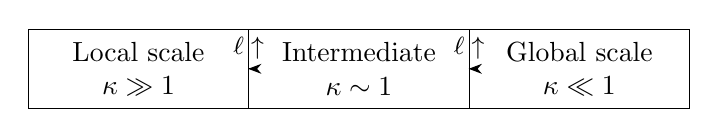
\begin{tikzpicture}[node distance=2.8cm, >=Stealth]
\node[draw,rectangle,minimum width=2.8cm,minimum height=1cm,align=center] (local)  {Local scale\\ $\kappa \gg 1$};
\node[draw,rectangle,minimum width=2.8cm,minimum height=1cm,align=center] (mid)    [right of=local]  {Intermediate\\ $\kappa \sim 1$};
\node[draw,rectangle,minimum width=2.8cm,minimum height=1cm,align=center] (global) [right of=mid]    {Global scale\\ $\kappa \ll 1$};
\draw[->] (local) -- (mid) node[midway,above] {\small $\ell\uparrow$};
\draw[->] (mid) -- (global) node[midway,above] {\small $\ell\uparrow$};
\end{tikzpicture}
\caption{Renormalization flow from coherent local regimes toward turbulent global instability. Increasing scale degrades correction capacity relative to entropy production, driving $\kappa \to 0$.}
\end{figure}

\subsection{Algorithmic Amplification as Scale Acceleration}

Modern dissemination systems act as operators that effectively compress renormalization steps:
\[
\ell \rightarrow \ell_{\text{eff}} \gg \ell.
\]

This applies a coarse-graining transformation without the intermediate stabilization that occurs under natural diffusion, driving the system directly into the turbulent regime. Algorithmic amplification is not merely increased visibility but accelerated renormalization. Inequality under scale change is similarly non-uniform: high-resource agents maintain $\beta(\ell)\mathcal{C}(\ell)$ relatively stable, while low-resource agents experience rapid decay, producing $\kappa_i(\ell) \gg \kappa_j(\ell)$ for large $\ell$.

\begin{theorem}[Renormalization Form of the No-Go Theorem]
Under increasing scale, the renormalization flow drives the stability ratio to zero:
\[
\ell \uparrow \quad \Rightarrow \quad \kappa(\ell) \downarrow \rightarrow 0.
\]
Stable high-visibility operation cannot be maintained across arbitrarily large scales.
\end{theorem}

\begin{proof}
By the scale dependence of parameters, $\alpha(\ell)/\beta(\ell) \uparrow$ and $|\nabla\Phi_\ell|^2 \uparrow$ as $\ell$ increases while $\mathcal{C}(\ell)$ does not compensate. Therefore $\kappa(\ell) \to 0$. \hfill$\square$
\end{proof}

\section{Visibility as a Relevant Operator}

We complete the field-theoretic account by classifying visibility within a renormalization framework as a perturbation whose influence grows under scale transformation.

\subsection{Operator Classification and Growth}

Under the scale transformation $x \to \lambda x$, the visibility field transforms as $\Phi(x) \to \lambda^{\Delta_\Phi}\Phi(\lambda x)$. Operators are classified as relevant ($\Delta_\Phi > 0$), marginal ($\Delta_\Phi = 0$), or irrelevant ($\Delta_\Phi < 0$). Visibility behaves as a relevant operator: $\Delta_\Phi > 0$, meaning
\[
\Phi_\ell \sim \ell^{\Delta_\Phi}, \qquad \frac{d\Phi}{d\log\ell} > 0.
\]

Because entropy production scales as $|\nabla\Phi|^2$, the growth of $\Phi$ under renormalization induces superlinear entropy growth:
\[
S_\ell \sim \ell^{2\Delta_\Phi}.
\]

Visibility is therefore not only relevant but entropy-amplifying under scale change.

\begin{figure}[htbp]
\centering
\begin{tikzpicture}[scale=1.1]
\draw[->] (0,0) -- (5.5,0) node[right] {scale $\ell$};
\draw[->] (0,0) -- (0,4.5) node[above] {$\Phi(\ell)$};
\draw[thick,domain=0:4.5,samples=80] plot (\x, {0.12*\x*\x + 0.3*\x + 0.3});
\node[right] at (4.5,2.6) {\small relevant growth $\Phi \sim \ell^{\Delta_\Phi}$};
\draw[dashed] (0,1.2) -- (5,1.2) node[right] {\small marginal};
\end{tikzpicture}
\caption{Visibility as a relevant operator: $\Phi(\ell)$ grows under scale transformation while a marginal operator would remain constant. The superlinear growth drives entropy production and instability at large scales.}
\end{figure}

\subsection{Fixed Points and Irreversibility}

Two qualitative fixed points are identifiable. The coherent fixed point $(\Phi \approx 0, S \approx S_0, \kappa \gg 1)$ corresponds to low coupling and stable interpretation. The turbulent fixed point $(\Phi \gg 1, S \gg 1, \kappa \ll 1)$ corresponds to maximal coupling and loss of coherence. The relevance of visibility drives the system away from the coherent fixed point toward the turbulent one. Because $\sigma \geq 0$, this flow is not symmetric: once the system has been driven toward high entropy, returning to the original fixed point requires external work. Visibility is therefore not only relevant but irreversibly relevant.

Suppression of this relevance requires reducing the effective scaling dimension $\Delta_\Phi$, increasing $\beta(\ell)$, or partitioning the manifold to prevent global coupling. These correspond precisely to the practical strategies of selective dissemination, domain restriction, and reputation buffering.

The classification of visibility as a relevant operator completes the field-theoretic interpretation of publicity. Virality is the natural consequence of a perturbation that grows under renormalization flow. The ideology of maximizing visibility is equivalent to applying a relevant operator that drives the system to a high-entropy fixed point. Without structural modification of the scaling behavior, the flow toward instability is not contingent but thermodynamically inevitable.

\section{Conclusion: Coherence Under Flow}

\begin{figure}[htbp]
\centering
\begin{tikzpicture}
\draw[->] (0,0) -- (6.5,0) node[right] {flow (exposure)};
\draw[->] (0,0) -- (0,4) node[above] {coherence};
\draw[thick] (0,3.5) -- (6,2.8) node[right] {\small controlled};
\draw[thick,dashed] (0,3.5) .. controls (2,2.5) and (4,1.2) .. (6,0.4) node[right] {\small virality};
\draw[dotted] (3.2,0) -- (3.2,3.1);
\node[below] at (3.2,0) {\small $\Phi_c$};
\end{tikzpicture}
\caption{Coherence under flow. Controlled dissemination (solid) maintains coherence across increasing exposure. Indiscriminate virality (dashed) causes coherence to collapse past the critical threshold $\Phi_c$. The invariant to be preserved is not the amplitude of the signal, but the integrity of the structure that carries it.}
\end{figure}

The foregoing analysis reveals a unified structure beneath phenomena that ordinarily appear unrelated: gossip in offline communities, competitive suppression in markets, resentment in curved grading systems, algorithmic containment of disruptive ideas, and the contested question of whether a decentralized AGI ecology could sustain stable high-visibility operation.

In each case, the underlying mechanism is the same. An agent increases its coupling to a heterogeneous field. The field generates flows. The flows produce entropy. The entropy accumulates faster than it can be corrected. The signal degrades.

The question posed by the AGI extension is whether these dynamics are contingent features of current systems or structural properties of any system operating under distributed interpretation. The analysis suggests the latter. The No-Go Theorem holds under assumptions that are not specific to human social systems: interaction produces distortion, visibility induces interaction, and correction is bounded. Any system operating on a heterogeneous manifold with finite corrective capacity faces the same constraints. What changes across system types is the magnitude of the parameters, not the form of the inequalities.

The four-phase structure---coherent, competitive, turbulent, resonant---provides a map of the possible regimes, and the order parameters $(\kappa, \eta, \chi)$ provide the coordinates. Human social systems typically oscillate between Phases I and III. Current platforms tend to drive systems toward Phase III. The AGI vision targets Phase IV. Whether Phase IV is accessible, and whether it remains stable once reached, depends on whether the thermodynamics of interpretation can be genuinely re-engineered or whether the entropy production term reasserts itself at larger scales and longer timescales.

The lesson is not that communication is impossible or that exposure should be avoided entirely. It is that visibility is a dynamical variable with costs, not a monotonically good quantity to be maximized. The rational strategy under these dynamics is to achieve objectives with the least exposure necessary, preserving structural integrity under adversarial and entropic flows.

Within the RSVP framework, this is not a sociological observation but a consequence of field geometry. The reputational sector instantiates the same scalar--vector--entropy coupling that governs any non-equilibrium plenum. Coherence under flow is the invariant that must be preserved. Virality is its destruction.

The problem of publicity is therefore not one of amplification but of stability. And stability, in any field-theoretic system, is achieved not by increasing the amplitude of the signal, but by maintaining the integrity of the structure that carries it. Whether any successor system---artificial, hybrid, or otherwise---can sustain that integrity at the scales it would need to operate remains, within this framework, the central open problem.

\newpage

\begin{thebibliography}{99}

\bibitem{shannon1948}
C. E. Shannon,
\textit{A Mathematical Theory of Communication},
Bell System Technical Journal, 27(3), 379--423 (1948).

\bibitem{cover2006}
T. M. Cover and J. A. Thomas,
\textit{Elements of Information Theory},
Wiley-Interscience (2006).

\bibitem{prigogine1977}
I. Prigogine,
\textit{Time, Structure, and Fluctuations},
Science, 201(4358), 777--785 (1977).

\bibitem{haken1983}
H. Haken,
\textit{Synergetics: An Introduction},
Springer (1983).

\bibitem{anderson1972}
P. W. Anderson,
\textit{More is Different},
Science, 177(4047), 393--396 (1972).

\bibitem{castells1996}
M. Castells,
\textit{The Rise of the Network Society},
Blackwell (1996).

\bibitem{barabasi1999}
A.-L. Barabási and R. Albert,
\textit{Emergence of Scaling in Random Networks},
Science, 286(5439), 509--512 (1999).

\bibitem{watts2002}
D. J. Watts,
\textit{A Simple Model of Global Cascades on Random Networks},
Proceedings of the National Academy of Sciences, 99(9), 5766--5771 (2002).

\bibitem{vosoughi2018}
S. Vosoughi, D. Roy, and S. Aral,
\textit{The Spread of True and False News Online},
Science, 359(6380), 1146--1151 (2018).

\bibitem{sunstein2009}
C. R. Sunstein,
\textit{On Rumors: How Falsehoods Spread, Why We Believe Them, What Can Be Done},
Farrar, Straus and Giroux (2009).

\bibitem{girard1977}
R. Girard,
\textit{Violence and the Sacred},
Johns Hopkins University Press (1977).

\bibitem{bourdieu1986}
P. Bourdieu,
\textit{The Forms of Capital},
in \textit{Handbook of Theory and Research for the Sociology of Education} (1986).

\bibitem{goffman1959}
E. Goffman,
\textit{The Presentation of Self in Everyday Life},
Doubleday (1959).

\bibitem{debord1967}
G. Debord,
\textit{The Society of the Spectacle},
Buchet-Chastel (1967).

\bibitem{tversky1974}
A. Tversky and D. Kahneman,
\textit{Judgment under Uncertainty: Heuristics and Biases},
Science, 185(4157), 1124--1131 (1974).

\bibitem{ashby1956}
W. R. Ashby,
\textit{An Introduction to Cybernetics},
Chapman \& Hall (1956).

\bibitem{wiener1948}
N. Wiener,
\textit{Cybernetics: Or Control and Communication in the Animal and the Machine},
MIT Press (1948).

\bibitem{bertalanffy1968}
L. von Bertalanffy,
\textit{General System Theory},
George Braziller (1968).

\bibitem{smale1967}
S. Smale,
\textit{Differentiable Dynamical Systems},
Bulletin of the American Mathematical Society, 73(6), 747--817 (1967).

\bibitem{strogatz2015}
S. H. Strogatz,
\textit{Nonlinear Dynamics and Chaos},
Westview Press (2015).

\bibitem{goertzel2014}
B. Goertzel,
\textit{Artificial General Intelligence: Concept, State of the Art, and Future Prospects},
Journal of Artificial General Intelligence, 5(1), 1--48 (2014).

\bibitem{goertzel2020}
B. Goertzel,
\textit{The AGI Revolution: An Inside View of the Rise of Artificial General Intelligence},
World Scientific (2020).

\bibitem{minsky1986}
M. Minsky,
\textit{The Society of Mind},
Simon \& Schuster (1986).

\bibitem{ostrom1990}
E. Ostrom,
\textit{Governing the Commons},
Cambridge University Press (1990).

\bibitem{nowak2006}
M. A. Nowak,
\textit{Five Rules for the Evolution of Cooperation},
Science, 314(5805), 1560--1563 (2006).

\bibitem{axelrod1981}
R. Axelrod and W. D. Hamilton,
\textit{The Evolution of Cooperation},
Science, 211(4489), 1390--1396 (1981).

\bibitem{friston2010}
K. Friston,
\textit{The Free-Energy Principle: A Unified Brain Theory?},
Nature Reviews Neuroscience, 11(2), 127--138 (2010).

\bibitem{deco2011}
G. Deco, V. Jirsa, and A. McIntosh,
\textit{Emerging Concepts for the Dynamical Organization of Resting-State Activity},
Nature Reviews Neuroscience, 12(1), 43--56 (2011).

\bibitem{newman2010}
M. E. J. Newman,
\textit{Networks: An Introduction},
Oxford University Press (2010).

\bibitem{rogers2003}
E. M. Rogers,
\textit{Diffusion of Innovations},
Free Press (2003).

\bibitem{barton2025}
J. Barton,
\textit{Coherence Thermodynamics: Structure from Contradiction},
Preprints (2025),
\texttt{doi:10.20944/preprints202507.1448.v3}.

\end{thebibliography}

\end{document}
